\documentclass[12pt]{report}
\usepackage{gensymb}
\usepackage{lineno}
\usepackage{titlesec}
\usepackage{geometry}
\usepackage{lipsum}
\usepackage{caption}
\usepackage{subcaption}
\newgeometry{
    top=1in,
    bottom=1in,
    outer=1in,
    inner=1in,
}
\usepackage{setspace} \doublespacing
\titleformat*{\section}{\LARGE\bfseries}
\titleformat*{\subsection}{\Large\bfseries}
\titleformat*{\subsubsection}{\large\bfseries}
\usepackage{hyperref}
\hypersetup{%makes links, references, and table of contents hyperlinks within the text, and colours them blue
    colorlinks,
    citecolor=blue,
    filecolor=black,
    linkcolor=blue,
    urlcolor=black
}
\usepackage{graphicx}
\usepackage[english]{babel} 
\usepackage[
backend=biber,
style=numeric,
sorting=ynt
]{biblatex}
 
\addbibresource{mybibliography.bib}
\begin{document}
\begin{titlepage}
    \begin{center}
        \vspace*{0.5cm}
        
        \large
        \textbf{Highly Sensitive Atomic Magnetometer For nEDM Experiment }
        
        \vspace{0.5cm}
        \large
        
        
        \vspace{1.5cm}
        by\\
        \vspace{0.9cm}
        Moushumi Das
        \vfill
        
% * <moushumi.das.phy@gmail.com> 2018-09-10T15:56:34.828Z:
%
% ^.
       \vspace{1.5cm}
       A thesis submitted to the Faculty of Graduate Studies of\\ The University of Manitoba\\
       in partial fullment of the requirements of the degree of\\
        \vspace{1.2cm}
        MASTER OF SCIENCE
        \Large
        \vspace{0.8cm}
        
        
\includegraphics[width=0.4\textwidth]{university_logo_}\\
        \large
        Department of Physics and Astronomy\\
        University of Manitoba\\
        Winnipeg
  
        
    \end{center}
\end{titlepage}



\begin{abstract}
%% Text of abstract
A non-zero neutron electric dipole moment (nEDM) would indicate time reversal and charge-parity violation (T and CP). Many experiments are currently being conducted or planned to measure the nEDM. At present the experimental upper bound on the nEDM is $3.0 * 10^{-26}$ e-cm. Our collaboration is developing an experiment at TRIUMF to improve the sensitivity to the nEDM by one order of magnitude ($10^{-27}$e-cm). I am proposed to develop a highly sensitive nonlinear magneto-optical rotation (NMOR) based magnetometer which is a crucial tool in the nEDM apparatus, for stability and homogeneity measurements. The NMOR magnetometer is designed to serve in an array of such sensors to form an auxiliary magnetometer system monitoring the stability and uniformity of the magnetic field in nEDM experiment at the TRIUMF. A NMOR magnetometer has been developed and constructed at the University of Winnipeg. In this NMOR system an atomic vapour cell containing natural rubidium with stable isotopes Rb-87 and Rb-85 is used. An NMOR resonance occurs when the optical pumping is synchronous with Larmor precession. This causes an atomic vapor to become dichroic, so that subsequent probe light experiences polarization rotation modulated at the same frequency. Currently I am working on testing the performance of this NMOR magnetometer.

\end{abstract} 
\pagestyle{plain}
\setcounter{page}{1}
\pagenumbering{roman} 
\tableofcontents
\newpage
\listoffigures
\newpage
\Large
\setcounter{page}{1}
\pagenumbering{arabic}
% page 1 % 
\chapter{Introduction }
\small
 \section{Neutron electric dipole moment and CP violation } 
 Neutron has an intrinsic electric dipole moment (EDM). The neutron EDM is a measure for the distribution of positive and negative charges inside the neutron. Intrinsic EDM of neutron interacting with external magnetic and electric fields can be described by the following Hamiltonian:
\begin{equation}\label{my_first_eqn}  
  H=-\mu_n.B-d_n.E
\end{equation}
where $\mu_n$ is the magnetic moment of the neutron interacting with the magnetic field B,and $d_n$ is the electric dipole moment of the neutron interacting with the electric field E.
\begin{table}[h]
\centering
\begin{tabular}{|l| l| l |l |}
\hline

\textbf{} & \textbf{C} & \textbf{P}  & \textbf{T}\\
\hline
$\mu_n$ & - & + & - \\
\hline
$d_n$  & -  & + & -  \\
\hline
$B$    & -  & + & -  \\
\hline
$E$    & -  &  - & +  \\
\hline
\end{tabular}
\caption{Symmetry properties of different components of the EDM Hamiltonian}
\end{table}
Table 1.1 describes the behavior of different component of Hamiltonian under discrete symmetries. According to this, the first term( $\mu_n.B$) is CP-even and T-even and the second term ($d_n.E$) is CP-odd and T-odd. Because of the conservation of CPT symmetry, A non-zero electric dipole moment of the neutron would be a violation of parity (P) and time-reversal (T) symmetry.

\section{nEDM measurement principle (Ramsey's method of separated oscillatory fields)}
\bigskip
In the nEDM experiment, spin-polarized ultracold neutrons, oriented along a uniform field $B_0$ stored into a neutron storage chamber. After applying the magnetic field $B_0$ along the z-axis of the storage cell, the ultra-cold neutrons start to precess about magnetic field $B_0$ at their Larmor frequency.  Then a radio frequency pulse at the Larmor frequency of the neutron is applied to flip the spin by $90 \degree$. The applied electric field is in a collinear orientation to B.
For parallel orientation of E and B, the rotational frequency becomes
\begin{equation}\label{my_first_eqn}  
    h{\omega_0}^ {\uparrow\uparrow}=2\mu_n {B}^{\uparrow\uparrow}+ 2 d_nE
\end{equation}
            
and for the antiparallel orientation of E and B, the rotational frequency is given by
\begin{equation}\label{my_first_eqn}  
    h{\omega_0}^ {\uparrow\downarrow}=2\mu_n {B}^{\uparrow\downarrow}- 2 d_nE
\end{equation}

where $\mu_n$ denotes the neutron magnetic moment, and $d_n$ denotes the hypothetical electric dipole moment
When the value of nEDM is zero, the neutron spin orientation will be anti-parallel to the initial spin orientation but the spin orientation will no longer antiparallel for non-zero nEDM. A fully magnetized Fe-foil is used to detect the neutron spin while transmitting the neutron from neutron chamber which is used to get information about spin orientation. The probability of neutron transmission is proportional to the neutron spin projection on the preferred direction of the Fe-foil. A neutron counter is used to detect the transmitted UCNs. A spin flipper is used to flip the remaining UCNs in the storage chamber in the preferred direction and then they are passed through the neutron counter. An incident for the nEDM is determined from the ratio of the counting rates.
\section{Comagnetometer}
\section{Origin of False EDM}
\section{Internal Magnetometry Impact on nEDM}
\newpage
\LARGE
\chapter{Atomic Magnetometry}
\small

 In the following chapter, there will be given an introduction into the quantum mechanical
structure and interactions of a Cesium atom with special focus on the hyperfine structure and the Zeeman splitting of the energy levels in an external magnetic field. In the second section of this chapter, the principle of atom-light interactions including optical pumping
will be explained. After introducing basic concepts of alkali atom quantum mechanics, the phenomenology of nonlinear magneto-optical rotation (NMOR) will be discussed, which is the basis for the operation of an atomic magnetometer as it will be used for the nEDM setup

\section{Ground state structure of Rb }
\label{S:2} 
Alkali-metal atoms have single electron in their outer shell. For this reason they are often used for optical pumping.Alkali-metal atoms have a nuclear spin,
which complicates their level structure.Because of the nuclear spin the energy level of these alkali atom becomes complicated.For example rubidium has Z = 37 where the first 36 electrons are in closed sub-shells and so their total angular momentum is zero. 
The ground state structure of the Rb atom is n = 5, l =0(s-state), and j = 1/2, i.e $5^2S_{1/2}$ .The lowest excited states(l =1) are the
 5p states. According to quantum theory of angular momentum
these 5p states have total electron angular momentum J = L + S where L is
the orbital angular momentum and S is the electron spin angular momentum.For the $5^2S_{1/2}$ and $5^2P_{1/2}$ states of 85Rb, which has nuclear angular momentum I = 5/2, the allowed values of F are $5/2$ - $1/2$ = 2 and 5/2 + 1/2 = 3.When atoms absorb light, they must absorb both energy and angular
momentum in the transition from the ground state to an excited state.The $5^2P_{1/2}$
state is separated from the $5^2S_{1/2}$ state by an energy corresponding to 795 nm wavelength, it is called the
D1 line. Transmission corresponding to the energy difference between the $5^2S_{1/2}$ and $5^2S_{1/2}$ levels of rubidium is termed the D2 line; its wavelength is roughly 780 nm\cite{doe:website}. For a D1-transition, the excited state F can occupy the states $F = 2$ or $F = 3$.
The U of Winnipeg Rb atomic- magnetometer is based on exciting the D1-line transition by optical pumping.  Linearly polarized laser beam is used to induce transitions of electrons from one energy level to another via optical pumping. In this case, the laser beam is tuned to the transition frequency and of sufficient power to perturb the equilibrium distribution of the ground state energy levels\cite{}. A linearly polarized probe beam propagating parallel to the
pump beam. After passing through the alkali vapor, the plane of polarization of the probe beam
rotates by an angle proportional to the spin component along that direction, and we detect
this rotation in order to observe the spin behavior.



\section{Atom-light interaction} 

In this section, an introduction into the principle of atom-light interactions will be given. Starting with different polarization modes of laser light and their impact on optical pumping, the concept of frequency /amplitude modulation of the pump laser light will be given.

\subsection{Polarization of laser light} 
There are three possible polarization states for a light wave, which refer to the behavior of the electric field vector ~E of the light. The three polarization states are illustrated in

\begin{itemize}
\item Circularly polarized light

In circularly polarized light, the vectors components Ex and Ey are perpendicular with respect to each other at each point in time(phase shift $\Delta$ = 90\degree.The magnitudes of the vector components are equal ($E_x = E_y$). Looking directly at the origin of the light, the electric field vector components Ex and Ey move on a circle while E is rotated by 360\degree within one wavelength. By pointing with the left-hand thumb into the direction of the source (against the direction of light propagation), the curl of the fingers indicates the left- or right-handed light polarization. Left circularly polarized light is also called $ \sigma^+$ light wh
ere a single photon carries an angular momentum of +1, while right circularly polarized light is usually called $\sigma^-$ light and carries an angular momentum of -1.
\medskip
right-handed circularly polarized light can be described by
\begin{equation}
     E(z,t)=\frac{E_0}{\sqrt{2}} \cos⁡(kz-\omega t)e_x+\frac{E_0}{\sqrt{2}}  \sin ⁡(kz-\omega t)e_y
\end{equation}
and left-handed circularly polarized light can be described by
\begin{equation}
     E(z,t)=\frac{E_0}{\sqrt{2}} \cos⁡(kz-\omega t)e_x-\frac{E_0}{\sqrt{2}} \sin⁡ (kz-\omega t)e_y
\end{equation}
\end{itemize}
\begin{itemize}
\item Linearly polarized light

In linearly polarized light, the electric field vector components  and  have a phase shift of $0 \degree$ or $360\degree$, which means that Ex and Ey oscillate in phase. Looking at the source of the light, the oscillation of E takes place at a certain plane. Linearly polarized light is a combination of equal fractions of left- and right-handed circularly polarized light. A single photon can thus transfer zero units of angular momentum. 
\begin{equation}
     E(z,t)=\frac{E_0}{\sqrt{2}}〖\cos〗⁡〖(kz-\omega t)e_x-\frac{E_0}{\sqrt{2}}〖\cos〗⁡〖(kz-\omega t〗)e_y
\end{equation}
\end{itemize}
\begin{itemize}
\item Elliptically polarized light

In the case of elliptical polarized light, the phase difference between Ex and Ey is non-zero. Furthermore, the magnitudes of Ex and Ey are always different. This leads to a rotation of the electric field vector on an ellipse if looking at the light source.
\end{itemize}
\subsection{Optical pumping(need to edit)}
\bigskip
Optical pumping is a process in which light is used to modify the quantum state of the medium. This process can generate polarized ground states in atomic media. It is a nonlinear process since the light alters the optical properties of the medium as it goes through.In the case of optical pumping, polarized light is used to polarize atomic sample. According to quantum selection rules, certain atomic states are not allowed to interact with certain polarizations of light. These states are called Dark state. Transitions from or to such state are forbidden.  On the other hand, states that can interact with the light will become less and less populated. This will result in different occupations of the fascinating sublevels in the atom. Consider an example system of F= 1 to F =~0 transition.  Linearly polarized light can decompose into two counter-rotating circularly polarized components with the respective magnetic quantum number m= $\pm$ 1 related to F. The transferable angular momentum is +1 for left circular polarization, -1 for right circular polarization and 0 for any linear polarization. After absorbing these photons, atoms can make a transition to excited states while the probability of belonging to a particular hyperfine sublevel of the excited state depends on quantum mechanical calculations. Fluorescence occurs by emitting a photon and the atom returns to the ground state. By emitting a photon, the atom returns to the ground state. This process is known as fluorescence. Both processes occur simultaneously which causes the rearrangement of population among different hyperfine/ Zeeman ground state sublevels. For right circularly polarized light, a transition from the M = $\frac{-1}{2}$ (F) to the M = $\frac{1}{2} F' $ state can be excited if the laser light is tuned to the transition frequency and of enough light power to perturb the equilibrium ground state population of the electrons. Rabi frequency (R) describes the strength of the light-atom interaction. It gives the strength of the coupling between the incident light and the transition associated with it.
The Zeeman sublevels M = 1 shift in energy in the presence of magnetic field by an amount $gB/\hbar$ where g is the Lande factor and is the Bohr magneton. This Zeeman splitting therefore leads to resonance frequencies for light also shift in energy. The left circularly polarized light experiences refractive index +n and the refractive index for right circularly polarized light is -n. In this case, optical rotation arises due to the difference in the refractive index 
\begin{equation}
\label{eq:emc}
\phi = \pi(n_+-n_{-})\frac{l}{\lambda} \\
\end{equation}
where l is the length of the medium traversed and is the wavelength of light. On resonance, the rotation is related to the Zeeman shift in the M = 1 sub levels.
\begin{figure}[h]
\centering
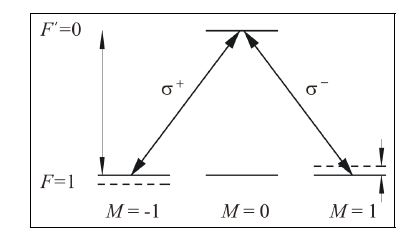
\includegraphics[width=0.75\linewidth]{optical_rotation}
\caption{Illustrative example of F = 1 to $F' = 0$ atomic transition with Zeeman
splitting in the presence of a magnetic field.Image\cite{Budker2002JU2}}
\end{figure}

\subsection{Magneto Optical Rotation}
\bigskip
In the presence of an axial magnetic field, when a linearly polarized light passes through an atomic medium the plane of polarization rotates. This kind of effect is known as the Faraday effect. When Larmor frequencies are smaller than the resonance linewidth, the produced optical rotation is directly proportional to the applied magnetic field which is the main feature of Linear Faraday rotation. We can relate this Faraday effect to the Zeeman shifts in the atomic energy level in the medium. The resonant enhancement of the Faraday rotation has discovered by D. Macaluso and O.M Corbino in 1898 which is known as nonlinear magneto-optical rotation (NMOR) or nonlinear Faraday rotation \cite{budker2013optical}. In the case of linear effect, optical rotation arises due to the absorption of certain contributions of the probe light. On the other hand, the generated disequilibrium in an atom via optical pumping gives rise to nonlinear effect which then alters the birefringent properties of a probe beam. 
As discussed above, the medium is optically pumped into an aligned state, which will
absorb y-polarized light, and not x-polarized light. This is linear dichroism, the differential absorption of orthogonal linear polarizations. On its own this would not affect our probe beam, as it is also polarized in the x-direction.The external B field now modifies the medium. The axis of alignment precesses in a
magnetic field, rotating the axis of dichroism.Finally, the probe beam interacts with the now rotated axis of dichroism, resulting in a rotation of polarization.
The optical rotation can be estimated as
\begin{equation}
\phi \approx \frac{(2g\mu B)/ \hbar\tau)}{(1+((2g\mu B)/(\hbar\tau))^2 )}\frac{l}{l_0}
\end{equation}
where $2g\mu/\hbar$ is correlated to Zeeman splitting, $\tau$ is the doppler width of the
absorption line (of order GHz), and $l_0$ is the absorption length in the medium. 
\begin{figure}
\centering
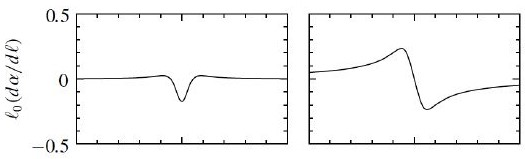
\includegraphics[width=0.85\linewidth]{faraday_rotation}
\caption{Optical rotation in the linear case\cite{auzinsh2010optically}}
\end{figure}
The aligned atoms relax after an average time 1/τ. In this time, how far around they precess depends on the magnetic field. As the field increases, the precession proceeds further and further, increasing the rotation. As the field becomes high enough to precess the alignment around a full revolution before it decays, the effect starts to average itself out over the ensemble of atoms, and the rotation decreases again. The symmetry of the shape comes from the fact that the precession goes the opposite way for a magnetic field of the opposite sign.
These two effects, the linear effect resulting from circular birefringence, and the nonlinear effect resulting from linear dichroism, represent the two basic mechanisms by which the polarization of the probe beam is rotated. In the zero field case these effects happen simultaneously and continuously, resulting in a steady signal being measured.


\section{Rb magnetometry based on NMOR}

The sensitivity of NMOR based atomic magnetometer depends on the lifetime of the polarization state. So in this case, it is important to use ground-state polarization since ground-state polarization has a longer lifetime than the excited states.The working principle of a Rb magnetometer can be described as three step process
\begin{itemize}
\item
Resonant  light polarizes Rb atoms via optical pumping. Magnetic moments of the atoms are oriented with respect to the axis of alignment
\end{itemize}
\begin{itemize}
\item Aligned magnetic dipole moments experience a torque and precess around the axis of the field at the Larmor frequency and medium becomes birefringent
\end{itemize}
\begin{itemize}
\item Optical polarization rotation of a probe beam is used to measure magnetic field
\end{itemize}
\begin{figure}[h]
\centering
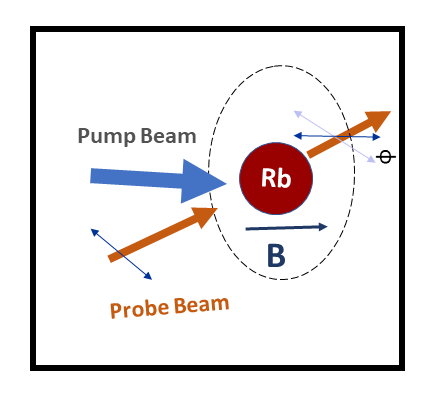
\includegraphics[width=0.55\linewidth]{optical_pumping}
\caption{The schematic diagram of the optical magnetometry technique.A linearly polarized pump beam is sent through the vapor cell containing natural Rubidium placed in a homogeneous magnetic field B .The polarization rotation of a linearly polarized probe beam is used to measure magnetic field}
\end{figure}
\chapter{Experimental setup}
\small

In this section, a general introduction into the experimental background of atomic magnetometry will be given. Starting with an explanation of the basic setup and its components, the dichroic atomic vapor laser lock (DAVLL), which is used for laser wavelength locking to the Cs absorption line will be discussed. Followed by an elucidation of the data acquisition (DAQ), this section will be completed with the comparison of different possible operation modes of an atomic magnetometer and an introduction into the concepts of magnetometer uncertainties and the noise level of a measurement
\section{Beam path}
 Figure 3.2 depicts the layout of the system used in the Physics Department of the University of Winnipeg for studying the non-linear magneto-optical effects with the amplitude modulated light. In this work, a paraffin-coated vapor cell (about 5 cm long) containing natural rubidium with stable isotopes $Rb^{87}$ and $Rb^{85}$, is used as the magneto-optical sample. To get maximum sensitivity and to reduce ambient fields the cell is placed within a magnetic shield made of four-layer of $\mu$ metal. This magnetic shield is capable to provide passive attenuation of dc magnetic fields by a factor of $10^6$. A semiconductor diode laser is the light source. The laser wavelength ($\lambda=795$ nm) is precisely controlled by an external locking system and its radiation is amplitude modulated by an acousto-optical modulator.  The light beam is splited into pump and probe beam using a beamsplliter. The typical light power of the pump beam is 40 $\mu$W and the typical light power of the probe beam is 20  $\mu$w. Upon passing through the Acousto Optic Modulator (AOM) and linear polarizer  linearly polarized light beam interact with Rb atoms. The probe beam then passes through our vapour cell which sits inside the shield. Then the nonlinear Faraday rotation signals are analyzed by a balanced polarimeter.  A Wollaston prism is used to split the beam into its perpendicular polarization axes which are then analyzed individually by our photodiode. Our photodiode contains two individual diodes and an internal differential amplifier which outputs the difference in diodes P1 - P2. A lock-in amplifier was used to detect the polarimetric signal and stored on a computer.
\begin{figure}[h]
\centering
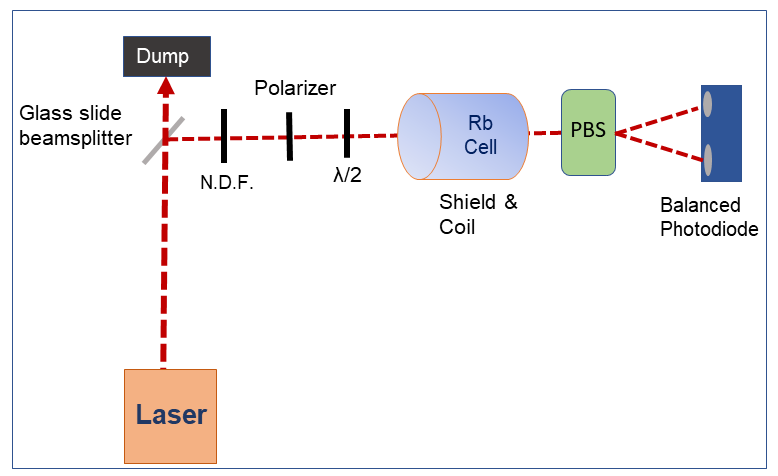
\includegraphics[width=1.1\linewidth]{experimental_setup_zero_field}
\caption{Schemetic diagram of experimental setup  for zero field NMOR measurement.}
\end{figure}
\begin{figure}[h]
\centering
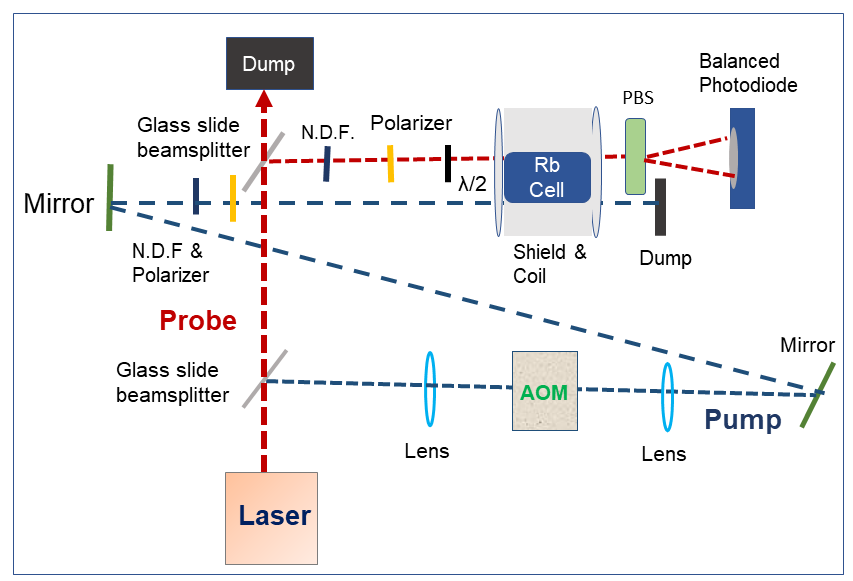
\includegraphics[width=0.95\linewidth]{experimental_setup}
\caption{Schematic diagram of the experimental setup for measuring rotation of the polarization plane with amplitude modulated(AM) light. AOM stands for acousto optic modulator, $\lambda/2$ - half wave plate, N.D.F- neutral density filter, PBS- polarizing beam splitter.}
\end{figure}
\section{External Cavity Diode Laser(ECDL)}
\bigskip
In our NMOR based optical magnetometry setup, laser light was provided by an external cavity diode laser. These kind of diodes are semiconductor diodes and thus vibration and shock resistant. They are also wavelength tunable. ’Besides that, external cavity diodes emit single mode laser light with a very narrow-band linewidth. A critical aspect of an ECDL is temperature control of the cavity, since the laser frequency depends on the cavity length and hence on the thermal expansion coefficient of the cavity material. Micrometer screws enable manual coarse tuning, while precise scans without mode hops are performed by a piezo actuator. This kind of grating stabilized diode lasers is especially advantageous for spectroscopy with the alkalines. Our Toptica DL-100 outputs a tunable wavelength near 795 nm with an output power $<100$ mW. The laser spot size is elliptical, and approximately 3 mm x 5 mm = $15 mm^2$.The laser was typically tuned to the D1 (F = 3,2 2) absorption minimum and then adjusted to maximize optical rotation. Our NMOR system uses an atomic vapour cell containing natural rubidium with stable isotopes $Rb_{87}$ and $Rb_{85}$ both being present.

\section{Dichroic Atomic Vapor Laser Lock (DAVLL)}
\medskip
In order to control the laser frequency to a fraction of the linewidth of the atomic transition of the Rb D1-line, a frequency error signal is generated by taking usage of the Zeeman effect combined with circular dichroism of an atomic vapor which is exposed to a magnetic field \cite{doi:10.1063/1.3568824}. The generated error signal passes through zero crossings as the laser frequency coincident with the lock frequency. A linearly polarized probe beam is incident on a glass cell filled with Rb vapor surrounded by a set of permanent magnets. The wavevector of the light is parallel to the axis of the generated magnetic field by permanent magnets. After the interaction of the laser beam with the Rb cell, the beam passes through a quarter-wave plate before impinging on a polarizing beam splitter (PBS) or a Wollaston prism. The linearly polarized beam incident can be split into two orthogonal circularly polarized beams. A set of photodiodes are used to detect the intensity of the right and left circularly polarized beams. Both of the photodiodes are attached to a polarimeter board which is used to measure the difference in signals and amplifies it. One oscilloscope is used for monitoring each photodiode as well as the difference output. The signal is then fed into a PID controller which finally controls the laser diode current corresponding to a certain laser frequency.
\begin{figure}[h]
\centering
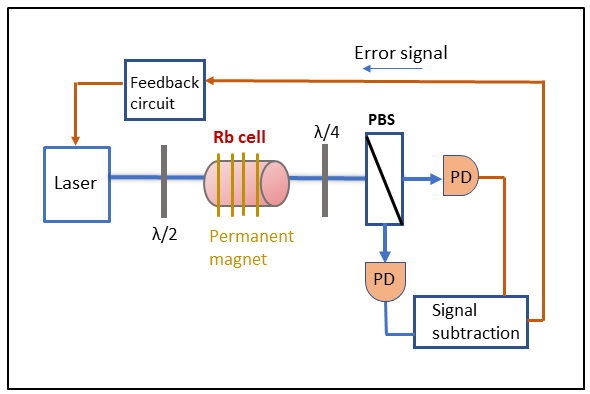
\includegraphics[width=0.8\linewidth]{DAVLL}
\caption{Schematic diagram of experimental setup for characterizing the DAVLL . PBS- polarizing beam splitter, PD- photodiode.}
\end{figure}
\section{Acousto-optic Modulator (AOM)}
Acousto optic modulator offer a method of modulating the light.This method works for both phase and amplitude modulation of light.In order to measure the magnetic fields in the far of the zero-field regime, an amplitude modulated pump beam needs to apply to the magnetometer.This amplitude modulation is done by a square wave modulation with a duty cycle of 1-10\%. This additional modulation is accomplished with an acousto optic modulator (AOM).
\begin{figure}[h]
\centering
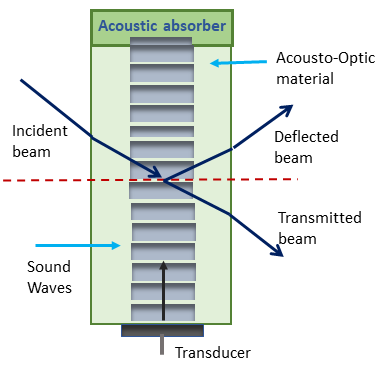
\includegraphics[width=0.7\linewidth]{AOM}
\caption{Acousto-optic modulator}
\end{figure}
In principle, it contains an optically transparent medium (e.g glass, quartz) which has a piezoelectric transducer attached at the end that propagates acoustic waves within the medium. An RF signal needs to apply to the transducer to generate the acoustic wave. The compressions and refractions of the sound waves result in periodic variations of the refractive index of the medium which then form a diffraction grating. Any incident laser beam will be diffracted by this grating generally provides a number of diffracted beams. The strength of the sound wave is directly related to the intensity of the defracted light. Depending on the interaction length L, laser wavelength $\lambda$ in the medium and the sound wavelength it is possible to operate AOM in two different modes: 
\begin{itemize}
\item  In the Raman-Nath regime ($L<\Lambda^2/\lambda$) many orders of diffraction are possible. The maximum intensity of the first-order diffracted light (relative to the incident light) is only about 35\%. Due to this relatively low efficiency, this type of AOM is used as a loss modulator fo r intracavity applications which require that light is removed from the zero-order diffraction or that a beam is straight propagating through the device e.g. Q-switching.


\end{itemize}
\begin{itemize}
\item In the Bragg regime($L > \Lambda^2/\lambda$) the light beam enters the medium at one particular Bragg angle 
\begin{equation}
\theta_B=\frac{\lambda}{2\Lambda}
\end{equation}                                 
and only one diffraction order produce. This observed diffraction pattern generally consists of two diffraction maxima; these are the zeroth and the first orders. In this case the possible maximum intensity of the first order diffracted light is 100\%. Due to this relatively high efficiency, this first order can be used for amplitude modulation. For our atomic magnetometry setup we operated the AOM in the Bragg regime.

For this prototype setup, an AOM driver is used with an RF center frequency of 80 MHz. The AOM uses crystal tellurium dioxide ($TeO_2$) for the optical interaction medium and Lithium Niobate as the piezoelectric transducer. The amplitude modulating pulses are driven with TTL signals, generated by an Agilent 33522A function generator. This AOM has a bandwidth of 80 MHz\\


\end{itemize} 
\section{Magnetic Shielding}
In precision magnetometry, magnetic shielding is required to achieve well characterized, stable magnetic field conditions independent of the earth’s magnetic fields and environmental perturbations. Shielding ratio T is a parameter to evaluate the efficiency of a shield which can be expressed as
\begin{equation}
 T = \frac{B_{in} }{B_0} 
\end{equation}

where $B_0$ is the homogeneous magnetic field in free space, and $B_{in}$ is the field induced in the presence of shield due to  $B_0$. Using multi-layer shielding is an efficient way to enhance shielding efficiency\cite{doe:website2} . The effectiveness of a multilayer shield with thin shells having wide gaps between them is same as the much heavier and more expensive thick, single layer shield.
The optimization of the air gaps between the shells is important to minimize the total size of a multilayer shield. When a coil is placed inside the innermost layer of passive shield the shield turns into a return yoke. As a result, the magnitude of field $B_0$ increase. A four layer $\mu$-metal magnetic shielding with nearly spherical geometry is used for this highly sensitive Rb magnetometer. $\mu$-metal is a very high permeability nickel based alloy, which is used for shielding low-frequency magnetic field. When the shape is close to a sphere we will get zero magnetic field inside independent of the outside field. The inner radius of the innermost shield is 18.44 cm, equal to its half-length. The radii and half-lengths of the progressively larger outer shields increase geometrically by a factor of 1.27. Each cylinder has two endcaps which possess a 7.5 cm diameter central hole\cite{Andalib:2016ahj}. A stove-pipe of length 5.5 cm is placed on each hole was designed to minimize leakage of external fields into the progressively shielded inner volumes. The magnetic shielding factors of each of the four cylindrical shells, and of various combinations of them, were measured and found to be consistent with $\mu_r \sim 20, 000$\cite{Martin:2014foa}
\begin{figure}[h]
\centering
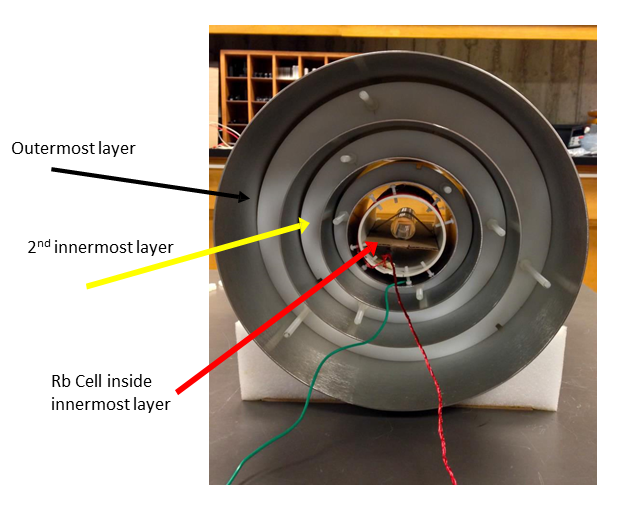
\includegraphics[width=1.0\linewidth]{magnetic_shielding}
 \caption{Four layer $\mu$ -metal magnetic shielding.The diameter of
each endcap is larger by 0.1 cm to fit over its corresponding cylinder. The hole diameter and stovepipe length for each endcap are the same. High
density polyethylene spacers and nylon thread rods/nuts are used to hold the shields and end caps together.}
\end{figure}
\newpage
\section{Rb Cell}
When glass cell is used to store alkali atoms, the atomic mean free paths increase and alkali spins depolarize immediately after making non-elastic collision with the glass walls.
Prolonging the atomic alignment is crucial to achieving ultra-narrow NMOR
resonance widths. So it is necessary to prevent these non-elastic collisions for achieving the longer lifetimes of atomic ground state coherences \cite{PhysRevA.72.023401}\cite{Balabas:10}  \cite{doi:10.1063/1.3236649}. Two methods are currently in use to extent the atomic coherence lifetime. One of them is to add buffer gas to the cell containing alkali sample and the other method is to coat the inner walls of the cell with anti-relaxation materials. The advantage of using buffer gas is that it reduces the resonance width by extending the lifetime of coherence state. A paraffin-coated vapor cell containing  natural rubidium with stable isotopes $Rb_{87}$ and $Rb_{85}$ is used for this work. The reason behind using paraffin as a anti-relaxation coating is that it allow polarized atoms to bounce off the walls of a paraffin-coated cell $\sim 1000$ times before depolarizing\cite{PhysRev.147.41}\cite{PhysRevA.72.023401}. Coated cells have the advantages of providing larger optical rotation
signals, reducing the effect of magnetic field gradients on the spin polarization lifetime,
and lowering the power requirements of the lasers used for pumping and probing. The vapor cell is cylindrical, 5 cm long and 5 cm in diameter with optical
flats on the ends. The cell was provided by D. Budker, having been prepared in
a fashion similar to the cells described in Ref.\cite{PhysRevA.72.023401}. The cell was characterized
using a method similar to Ref. \cite{PhysRevA.72.023401}, by measuring the relaxation of longitudinal
polarization using optical rotation as a probe. The long time component of the
relaxation was thereby found to decay with a time scale of 60 ms.  Longer relaxation time indicates good quality of cell. The temperature of the vapour cell was controlled by the ambient temperature of the surrounding room (∼ 21 $\deg$). Transmitted light was analyzed for optical rotation by a balanced polarimeter system containing a Wollaston prism and a Newport model 2307 balanced photo receiver. The power delivered to the vapour cell was typically 15 $\mu$W, measured periodically using a Newport Model 818-SL power meter inserted into the
beamline. 
\begin{figure}[h]
\centering
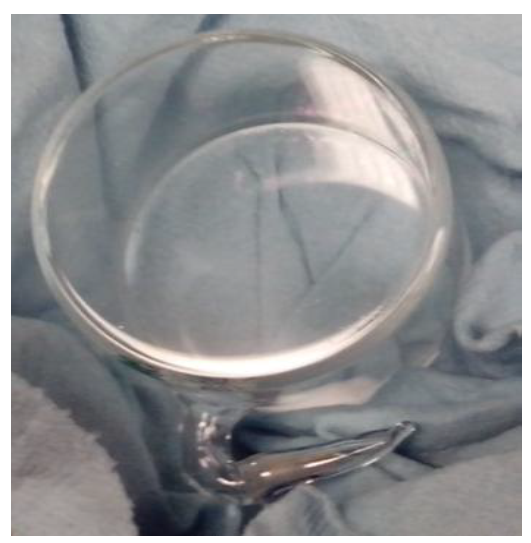
\includegraphics[width=0.5\linewidth]{cell}
\caption{Paraffin coated Rb cell}
\end{figure}
\newpage
\section{Internal coil}
 For the Rb atomic magnetometer an internal coil is used to provide the magnetic field. This coil produces uniform field in the ROI of magnetic shielding, directed along the axis of the cylindrical volume. The coil was wound on a 7.62 cm diameter, 20.32 cm long ABS plastic pipe. Seven turns of 26 AWG magnet wire were wound at 2.54 cm spacing, with 1.27 cm spacing from the magnetic faces of the endcaps of the innermost magnetic shield. The spacings were chosen so that, in the infinite permeability limit, and in the limit where the axial aperture holes in the endcaps are small, the boundary conditions would produce image currents forming an infinitely long solenoid . This is similar to the design strategy used in Ref. [16]. Two saddle coils were wound on the same cylinder in order to control transverse fields internally; these were normally disconnected during precision measurements. The internal coil system was calibrated using a three-axis fluxgate magnetometer at fields of ∼100 nT. This fluxgate was too large to fit through the end caps of the shield, so calibration
had to be performed without end caps. The calibration of the z-coil was verified using the NMOR magnetometer with an AM pump beam, and the known gyromagnetic ratios of Rb-85 and Rb-87. Homogeneity of the residual field and magnetic field generated by the coil system was measured by scanning a fluxgate magnetometer along the axis of the system with and without the coil energized. At a field of 1 $\mu$T, the axial field generated by the coil was uniform within the ROI to the $1\%$  level.
\section{Lock in Amplifier}
SR830 DSP Lock in Amplifier is a elementary part in the DAQ system of Rb magnetometry. It can measure very  small voltages. The most attractive feature of a lock in amplifier is that it is able to suppress all noise contributions which differ from the reference frequency. A reference signal is applied to the lock-in amplifier which is usually done by an external oscillator which passes a discriminator. In this magnetometry setup sync output of a function generator is used as external reference signal for force oscillation scan. The external reference signal is phase locked to an internal reference frequency, provided internal oscillator of the lock-in.Since a lock-in amplifier has two phase sensitive detectors we obtain two output signals. During the process of phase sensitive detection (PSD), the reference signal is first multiplied with the real input signal  and in a second stage, the real input signal is multiplied by
the lock-in reference signal with a phase shift of $90\degree$. Then a lowpass filter is used to filter both signals .The first one is referred to as X output and the 2nd output signal is referred to as Y output. X output is knows as in phase component and the Y output is called out of phase component.
\section{Degaussing system(need to edit)}
Our four layer $\mu$ metal magnetic shield is designed to minimize the magnetic field at the cell, but
magnetic hysteresis limits the magnetic field in any region to be exactly zero. Degaussing (demagnetizing) process is used to reduce the background magnetic field inside the shield. Although Rb cell is securely placed inside the four layer mu-metal shielding it is necessary to demagnetize the shield before every measurement session  to eliminate accidentally created local magnetizations.
Demagnetizing is achieved by winding a special coil around inner most layer of shielding  in toroidal configuration
and supplying the coil with oscillating current. An Agilent 3522A function generator  provides a ramped sinusoidal that controls a current supply driving the degaussing coil \cite{Martin:2014foa}. The wires going to the degaussing loop should be twisted together to avoid picking up or causing noise. Switch is opened to electrically disconnect the degaussing coil.
 
\begin{figure}[h]
\centering
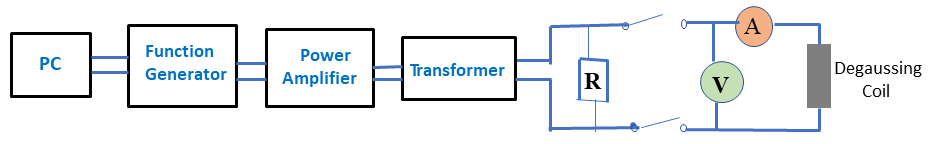
\includegraphics[width=1.0\linewidth]{degaussing_system}
\caption{Schematic diagram of degaussing System}
\end{figure}

\section{Signal Processing(need to edit)}
For small optical rotation, the rotation angle $\theta$ is given by 
\begin{equation}
\theta=\frac{p_1-p_2}{2(p_1+p_2)}
\end{equation}
       
where $P_1$ and $P_2$ represent signals of the two photodiodes in the polarimeter. The differential value is acquired with a lock-in amplifier (LIA) referenced to the pump beam modulation provided by a function generator. The demodulated signal from the LIA is acquired by a personal computer for analysis. 
\section{Laser tuning and locking}
In order to polarize atoms by optical pumping, it's important to tune the laser properly to expected transition line.
Setting the laser temperature correctly is one of the important parts to achieve good tuning . First we need to turn on the temperature control panel and then it’s easy to adjust laser temperature manually by tuning the knob of temperature control panel. For our tune the laser temperature is set to 20.1 $\degree C$. For good tuning it is also important to know the laser current which corresponds to the emission of laser light with a wavelength matching the absorption line of the Rb atom. This is usually done by a DAVLL scan so it's necessary to make sure the DAVLL optical setup is done correctly. An oscilloscope is used to observe the output of the differential amplifier. Trigger the scope on the trigger output on the sweep control panel.
Laser current can be controlled by adjusting the current control knob until the spectral structure of Rb -85 appears. we need to keep adjusting the current control knob until a maximum symmetry between the upsweep and downsweep portions is achieved. After that by adjusting the knob of sweep control panel we can zoom in the structure and set the trigger to steep of the absorption minima. 


Digilock 110 feedback controlyzer is used for laser locking. The DigiLock 110 is an up-to-date digital hardware allows to implement the scan generator, PID controllers and optional frequency modulation techniques all into one plug in module. It offers graphical user interface running on a PC makes the procedure of laser locking enormously easy. Different important features are also available in this module for analyzing and optimizing the control system.
 
The output of the laser feedback controlyser panel is connected to the computer where Digilock software was already installed. The output signal of the differential photodiode is fed into the controlyser panel main input. After connecting the DigiLock 110 we can turn on scan and navigate to the autolock screen at the bottom. Then the the portion of the spectrum that we tuned earlier will appear. Then we need to select the crosshairs tool which allow us to drag the crosshairs on the part of the spectrum that we want to tune to. Finally for successful laser locking we need to click and select "PID lock to slope".
\begin{table}[h]
\centering
\begin{tabular}{|l | l|}
\hline

\textbf{ Position}    & \textbf{Laser Power} \\
\hline

AOM &   $4mW$  \\

Pump beam   &    $60\mu W$  \\

Probe beam   &    $22\mu W$  \\
After Cell  &      $18\mu W$   \\

\hline
\end{tabular}
\caption{Adjusted laser power at several positions in the experiment}
\end{table}

\chapter{Rb magnetometer characterization at UW}
\section{Operation modes}

 In order to determine the maximum sensitivity,an magnetometer can be operated in different mode.An atomic
magnetometer is capable of magnetic field detection in any available operation modes. Most of them found its application during the time this Master's thesis was prepared.Although main focus of this work was to study magnetometer performance in Free Induction Decay (FID) mode.
 \subsection{Forced Oscillation Mode(need to edit)}

 In this force oscillation measurement scheme we modulate the drive frequency of amplitude modulated light and  observe the magnetometer response using a lock-in amplifier.A resonance scan using lock-in amplifier can be done by demodulating the signal at the drive frequency which are act as reference frequency.For this force oscillation scan a frequency range and frequency increments are entered into the DAQ software. Via a
GPIB connection, a function generator is set to the appropriate frequencies, driving
the pump modulation of the magnetometer. The frequencies are taken by the lock-in
amplifier as a reference signal as well as the differential output of the polarimeter board
which is demodulated at the reference frequency. The resulting X and Y outputs are sent to the DAQ program, running on a computer via GPIB. 
\begin{figure}[h]
\centering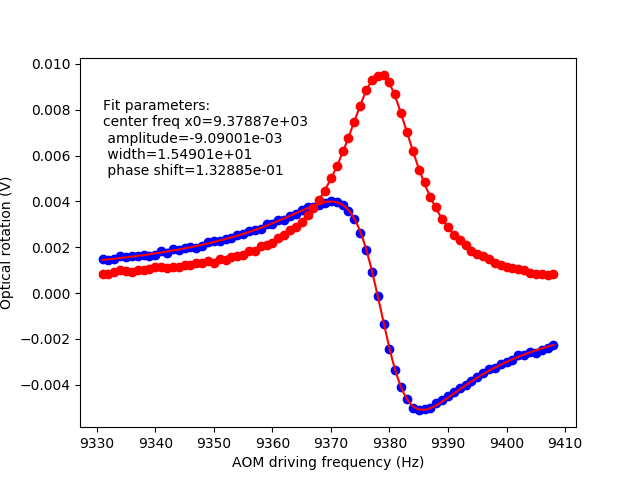
\includegraphics[width=0.4\linewidth]{FM_NMOR}
\caption{Optical rotation vs. forced oscillation frequency}
\end{figure}
The quadrature components arise because exactly on resonance, the aligned atoms produce maximum optical rotation when the alignment axis is at an angle of $ \pi/4$   to the direction of the light polarization.  
The probe beam then analyzed by photodiode whose output was connected to a digital-signal-processing lock-in amplifier.The lock-in is connected to a computer via GPIB. The DAQ computer saves the lock-in data in  a Python program where the data can be analyzed. The idea of the fitting algorithm is to generate a concatenated function, having the absorptive part as the first part and the dispersive as the second (directly connected to each other). The corresponding frequency values are simply the frequency scan range for the absorptive part while the frequency increments are added to the maximum frequency point of the absorptive in order to obtain the frequency parts for the dispersive curve. This results in
the overall data for the frequency, which is inserted into the fitting function.\\
The function of absorptive part can be expressed as:
\begin{equation}
\phi_y= \frac{A_0 (X-X_0 )\omega_0}{2(X-X_0 )^2+(\omega_0^2)/4}\cos\theta-\frac{\omega_0^2A_0}{(X-X_0 )^2+(\omega_0^2/4)}\sin\theta
\end{equation}
while the dispersive part of complex lorentzian is given by 
\begin{equation}
\phi_x= \frac{A_0 (X-X_0 )\omega_0}{2(X-X_0 )^2+(\omega_0^2)/4}\sin\theta+\frac{\omega_0^2A_0}{(X-X_0 )^2+(\omega_0^2/4)}\cos\theta
\end{equation}
In this conjunction, $A_0$ represents the maximum of the purely absorptive curve, $\omega_0$ the width
of resonance (FWHM) and $x_0$ the center resonance frequency. Furthermore, x represents
the frequency values.
The overall fitting function in order to really fit a complex lorentzian is given by (the
phases in R(x) and D(x) are not considered in the following equations, since they are varied
(sin/cos)).\\


\begin{equation}
F = R(x)^{'}\theta(x \leq f_{max}) + D(x-f_{max})^{'}\theta(x > f_{max})
\end{equation}
Where 
\begin{equation}
R(x)^{'}=R(x) . \cos(\phi_0) + D(x) .\sin(\phi_0)
\end{equation}\\
and
\begin{equation}
R(x)^{'}=D(x) . \cos(\phi_0) - R(x) .\sin(\phi_0)
\end{equation}

Here, $\phi_{0} $ represents the phase shift between the absorptive and dispersive parts. This phase shift$\phi_{0}$ appears due to the wrong settings of lock-in amplifier.The actual fitting function in equation 4.3 includes a case
structure, as it is given by the Heaviside-like function $\phi(x)$. If $ (x \leq f_{max}) $ ,$\phi(x)$ becomes zero,
if $(x > f_{max})$, it is equal to one. The initial guesses for the least-square parameters are given
as:\\
\begin{itemize}
\item
Amplitude $A_0$: In order to get guess amplitude, Averaging the maximum of the absorptive and dispersive curve is done.
\item
Width $\omega_0$: A width of the resonance curve of 15 Hz is assumed.
value.
\item
Center frequency $x_0$: The maximum frequency value of the
absorptive curve is considered as a guess for the center frequency.
\item
Phase $\phi_0$: In order to get a guess for the phase, $ R =\sqrt (
X^2 + Y ^2)$ is calculated for each
X and Y data pair. The corresponding X and Y data pair which gives the maximum
R value is taken and the phase guess $\phi _0$  is calculated by $\phi _0 = arctan(Y_{max}=X_{max})$.
\end{itemize}
Advantages: In the force oscillation scan technique entire resonance curve is scanned which allow us to see if there is a pure resonance or the real resonance curve get destroyed by any other external influences. By mapping out the entire resonance curve, we can easily debug the problem because in this process we can repeatedly adjust the power of the pump and probe beam immediately after each scan. Since the output signal of the balanced photodiode is demodulated stepwise by the lock-in amplifier at the modulation frequency at each increment, small amounts of noise induce in this process which is the most advantageous point of this field measurement technique. \\
Disadvantages: The force oscillation scan is a quite slow process which is the main drawback of this measurement scheme.
For a scan range of some hundred Hz usually takes a few minutes with  waiting time of couple second. As a result the force oscillation scans are not directly sensitive to magnetic field drifts, occurring at time intervals which are shorter than the actual scan. Field drifts would cause a degradation of the precision of a swept oscillation scan.
\subsection{Self oscillation mode}
In self-oscillating mode, the output signal of photodiode is  fed back to AOM for  amplitude modulation. In this case the  output signal of polarimeter is modified to act as a square wave which drives the AOM directly. After setting the phase and gain of the feedback system properly, the system start to oscillates spontaneously  at the Larmor frequency. In order to measure the oscillation frequency a frequency counter can be used in this mode. An online tracking of the oscillating signal is also possible.
 A customized circuit board, consisting of an analog voltage amplifier, a Schmitt trigger, and two metastable circuits, is used to process optical rotation \cite{PhysRevA.62.043403}.\\
Advantages: Being a quite fast process and having a high bandwidth are the main features of this self-oscillation scan. In order to get rapid update of the magnetic field the magnetometer can be operated in this mode.\\
 Disadvantages: Since feedback loop self-oscillate in the case of constructive interference, it will work only for the signal having a phase shift of integer multiple of $ 2\pi$. This additional phase shift might be resulting into slightly off-centered resonance. As a result, self-oscillation mode is more susceptible to systematic errors in field measurement.


\subsection{Free Indution Deecay(FID) }
\bigskip
\begin{itemize}
\item The magnetometer can also
be run in free induction decay mode,where Rb atoms inside the cell is excited once and afterwards the decaying processes of the excited atoms is observed. A function generator is used to delivered the pump pulses which are necessary for pumping during a FID measurement. The output frequency of the function generator is set to the resonance frequency
\item Pumping is done for a very short time interval and the coherence decay takes place fast. The pumping process is instantaneously stopped by AOM (by applying a digital TTL signal an acousto-optic modulator can be used to shutter a laser beam on and off), which can also be used to trigger the  data acquisition (DAQ). The change in the optical rotation of probe beam is measured by balanced  photodiode and the outpu signal of the photodiode is then fed into the lock-in amplifier.
\item The reference signal on the lock-in amplifier has further to be set slightly off resonance ($\sim 100 Hz$) in internal frequency mode in order to properly record the FID.
The X and Y channels output of the lock-in amplifier are further transfered to a Tektronix oscilloscope.An python script is used to transfer the data presented on the oscilloscope screen to computer for further analysis. The entire process of pumpimg and probing during a measurement cycle in FID mode  has shown in Figure 4.2. Rb atoms are pumped using amplitude modulated laser beam for 0.1 sec and then observed the spontaneous decay of excited atoms for another 0.2 sec while the pump beam was off. \\
Table 4.1 shows the function generator and lock-in amplifier settings for FID measurement.
\begin{table}[h]
\centering
\begin{tabular}{|l |l|}
\hline

\textbf{ SETTING}    & \textbf{VALUE} \\
\hline
Function generator &   \\
\hline
Frequency & 9.4kHz   \\

Waveform    &  Square  \\

Amplitude   &  $1V_{pp}$  \\
Offset  &       500 mV  \\
Phase       &    $0\degree$ \\
Trigger     &   Manual  \\
Burst       &    1000 cycle \\
Amplitude modulation & On \\
\hline
Lock-in amplifier &     \\
\hline
Lock in frequency     & 9.297 KHz \\
Time constant     &  $300\mu s$ \\
Sensitivity      &  500mV  \\
\hline
\end{tabular}
\caption{Setting for FID at $1\mu T$ field}
\end{table}
\begin{figure}[h]
\centering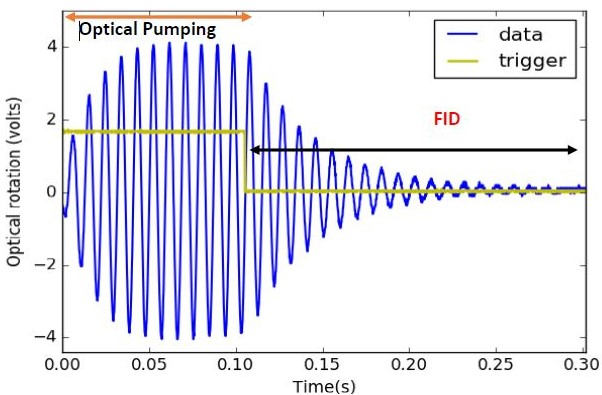
\includegraphics[width=0.55\linewidth]{Capture2}
\caption{ An example of Free Induction Decay(FID) signal, when pumping the Rb atoms  was done for 0.1 sec with linearly polarized light and probing was done for 0.2 sec.The applied magnetic field during the measurement is $0.2~\mu T$. }j
\end{figure}
The signal recorded  from X channel will be a sinusoid with an exponentially damping, according to   
  \begin{equation}
                                         y(t) = y_0 + A   e^{(t-t_0)/\tau}\sin(\omega t + \phi_0)
\end{equation}  

And the signal recorded  from Y channel will be a decaying cosine wave, according to
                                       
  \begin{equation}
                                         y(t) = y_0 + A   e^{(t-t_0)/\tau}\cos(\omega t + \phi_0)
\end{equation}
where $y_0$ describes a possible offset, A is the maximum amplitude of the sinusoidal oscillation,
t the present time, $t_0$ the starting point of the measurement, $\omega$ the oscillation frequency and $\phi_0$  some possible phase shift. The data fitting procedure were done in two ways in order to study a variety of systematic effects that were encountered. One method is to take a least square fit of x and y data separately to a decaying sin and cosine wave respectively. Another way of data fitting is to fit X and Y data simultaneously. A least square-fit of the recorded data set to equation (4.6) or (4.7) gives an estimate on frequency and  therefore the magnetic field.
\begin{figure}
    \centering
 
    \begin{subfigure}[b]{0.45\textwidth}
        \centering
        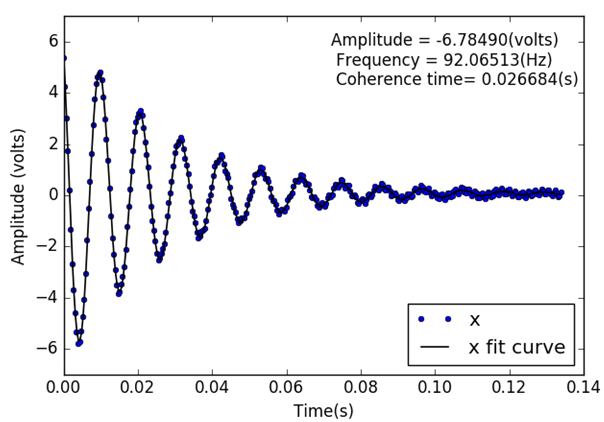
\includegraphics[width=\textwidth]{fid_x_fit}
        \caption{}
        \label{fig:three sin x}
    \end{subfigure}
    \hfill
    \begin{subfigure}[b]{0.45\textwidth}
        \centering
        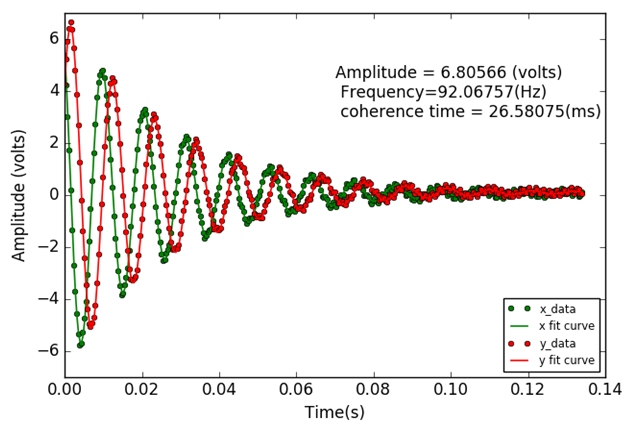
\includegraphics[width=\textwidth]{fid_simultaneous}
        \caption{}
        \label{fig:five over x}
    \end{subfigure}
    \caption{(a) Least square fit of X data(blue points are x data and black curve is fitted curve ) (b) Simultaneous fit of X and Y signal(green and red dots are represents x and y data respectively whereas green and red curve represents fit curves ) }
    \label{fig:three graphs}
\end{figure}

The initial guesses for the least-square parameters are given
as:
\begin{itemize}
\item
Beat frequency $\omega$: In order to guess the beat frequency, the Fast Fourier Transform (FFT) of FID signal is done.The extracted FFT frequency is used as guess frequency.
\item
Amplitude A: In order to get guess amplitude, Averaging the maximum of the X and Y data is done.
\item
Offset $\phi_0$: The mean of FID signal is calculated. This mean value is used as guess for the offset. 

\end{itemize}
The data fitting procedure provides us the actual value for those parameters. The oscillation frequency, one of the extracted fit parameters, is then is used to estimate the magnetic field according to the following equation
\begin{equation}
B= \frac{oscilation ~ frequency +~lock in~ frequency}{2\gamma}
\end{equation}
where $\gamma$ is the gyromagnetic ratio of Rb vapor. Figure 4.4 shows an example least square fit of FID signal where (a) represents only x output of lock-in amplifier and (b) represents both x and y output of lock-in.\\
Advantages: FID mode is free of probe and pump light induced light shifts because the optical pumping is done for a very short time period and the coherence decay process takes place quickly. 

Disadvantages: As a finite duty cycle is used (pump modulation only happens during a short period of time and the main idea is to watch the coherence decay, a decreasing of the maximum achievable sensitivity with this method.


\end{itemize}

\subsection{FID in tilted magnetic field}
For the nEDM experiment it is very important to do tilted field measurement in order to have better understanding of  geometric phase effects which are the leading sources for systematic uncertainties during nEDM measurement . 
Since our Rb magnetometer is a scalar magnetometer, it is not possible to measure vector field components directly.In general, when the magnetic field is along the light propagation direction, the main resonance occurs at $\Omega_m = 2\Omega_L$.This resonance appear because of the symmetry of the optically pumped state.It is found that When magnetic field direction is tilted in the plane perpendicular to the light polarization axis, resonance is observed at  $\Omega_m = 2\Omega_L$with its amplitude depending on the tilt angle.In this case, the amplitude of resonance signal decreases with increasing tilt angle . However, If we tilt the magnetic field direction towards the light polarization axis a new resonance appears at $\Omega_L$ along with the main resonance at $2\Omega_L$ if linearly polarized light is used.In this case the resonance signal contain two frequency component(Figure 4.3(a)) . The amplitude of the new resonance signal at $\Omega_L$  increases as the angle between B and the light propagation direction increases while main resonance amplitude at $2\Omega_L$  decrease with increasing tilt angle.However,when the tilt angle is larger than some certain angle the resonance amplitude measured at $\Omega_L$ also start to decrease and reaches zero when the magnetic field is directed along the y axis.   It could be possible to evaluate the magnitude of the magnetic field from the ratio of the resonance amplitudes at $\Omega_L$ and $2\Omega_L$.The same study with frequency modulated light has been reported by Pustelny et al.\cite{PhysRevA.74.063420}. In this study the NMOR Signal was observed by connecting the balanced photodiode to the oscilloscope directly. A python script is used to transfer the data presented on the oscilloscope screen to computer for further analysis. 

\begin{figure}
    \centering
 
    \begin{subfigure}[b]{0.45\textwidth}
        \centering
        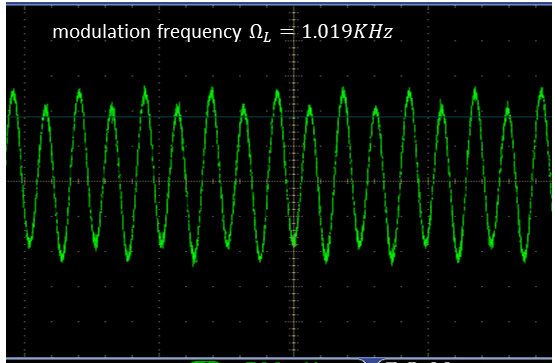
\includegraphics[width=\textwidth]{transverse_field}
        \caption{}
        \label{fig:three sin x}
    \end{subfigure}
    \hfill
    \begin{subfigure}[b]{0.45\textwidth}
        \centering
        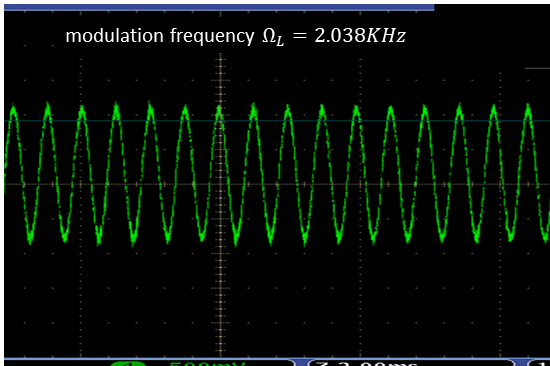
\includegraphics[width=\textwidth]{transverse_field_2}
        \caption{}
        \label{fig:five over x}
    \end{subfigure}
    \caption{(a) Optical rotation as a function of time at $\Omega_L$ in the yz plane at tilt angle $15\degree$ with light propagation direction. (b) Optical rotation as a function of time at $2\Omega_L$ for same tilt angle}
    \label{fig:three graphs}
\end{figure}


\chapter{Result}




\section{Study NMOR }
   \begin{itemize}
     \item NMOR near zero field \\
 During this measurement the pump beam was not been modulated. In this case,  at first degaussing the shields that surround the vapour cell is done in order to cancel background B-field.A function generator is used to drive the degaussing coil.After completing a degaussing sequence switch is opened to electrically disconnect the degaussing coil from experimental setup.Then B-field ramp is started and NMOR signal is observed through a oscilloscope which  connected to balance photodiode output.The magnetic field sweeping is done in a triangle wave.In figure (5.1) the whole sequence of measurement events has shown.The First secton of the scope trace has indicated to degaussing procedure,in 3rd section  switch was opened to disconnect the degaussing circuit from rest of the experimental setup, the 4th section describes the magnetic field($B_z$) sweeping. 
In this measurement NMOR signal is used to determine effectiveness of degaussing procedure.After the degaussing procedure the observed field inside the shield is non-zero while the applied field $B_z$ was zero which might indicate the existence of some remnant field.Durig this measurement the magnetic field ($B_z$) was ramped about 2.5 nT peak to peak which corresponds to resonance width 0.4 nT. The effect of degaussing parameter on resonance width will describe on section (5.6).
\begin{table}[h]
\centering
\begin{tabular}{|l |l|}
\hline

\textbf{ SETTING}    & \textbf{VALUE} \\
\hline
Function generator &   \\
\hline
Frequency & 10 Hz   \\

Sample rate    &  10000 sample/sec  \\

Amplitude   &  10 V \\
Offset  &       0 V  \\
\hline
\end{tabular}
\caption{Setting for degaussing }
\end{table}
     \begin{figure}[h]
 \centering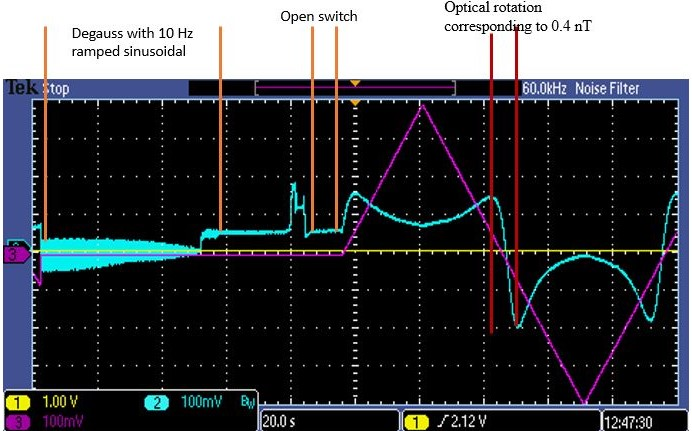
\includegraphics[width=0.7\linewidth]{scope_trace_of_field_sweeping}
\caption{Scope trace of total measurement scheme of NMOR near zero field.The purple curve shows that the magnetic field was ramped about $ 2.5 nT_{pp}$ with a triangular wave while the blue colored dispersive lorenzian shape curve indicate induced optical rotation due to field sweeping. }
\end{figure}
\newpage
In figure 5.2 NMOR data were acquired by sweeping the magnetic field in a triangle wave; the peaks in the curve show a slight dependence on the direction of the sweep, due to the time response of the atoms.The resonance width is about 0.49 nT.

 \begin{figure}[h]
\centering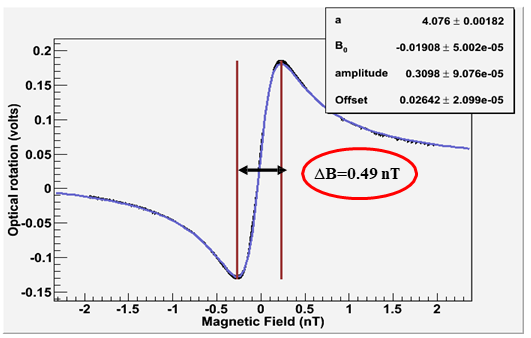
\includegraphics[width=0.7\linewidth]{near_zero_field}
\caption{Optical rotation as a function of magnetic field applied along the direction of the laser beam.The signal looks like a pure dispersive lorenzian curve.The measured resonance width is 0.49 nT}
\end{figure}
     \item Amplitude modulated magneto optical rotation(AM NMOR)\\
     To extent the magnetometer sensitivity to magnetic fields where Larmor precession is much faster than the ground state relaxation rate, it is necessary to synchronize the optical pumping rate with Larmor precession which can be achieved by modulating the light \cite{doi:10.1063/1.3225917}. In the case of AM NMOR, high-field resonance occur in addition to the regular zero-field resonance. The optical properties of the medium are being modulated at twice the Larmor frequency.In the case of strong external magnetic field, the dynamic Stark effect limits the sensitivity of NMOR based atomic magnetometry by reducing the accuracy of the field measurement. The advantage of using AM NMOR method is that it can reduce the Stark effect because light frequency is not affected by amplitude modulation\cite{gawlikoptical}. In AM NMOR, It is easily possible to control the number and amplitudes of the high field resonances by using the square wave modulation of light intensity.\\
In AM NMOR, we need to pump the atoms repeatedly, and a lock-in amplifier is used to observe the optical rotation at the same frequency. When this modulation frequency is the same as the harmonic frequency of the atoms we observe NMOR signal.During this study the reference frequency of lock-in amplifier is set to the modulation frequency.The x and y output signal of lock-in amplifier are shown in figure 5.3.The
black curve corresponds to the in-phase component(x), the red curve to the out of phase component(y).The dispersion structure(y component) is the resonance that can be observed in a regular rotation experiment with no modulation.  The modulation frequency of the pump beam was set to its resonance while the X and Y outputs recorded.In this case the observed resonance width is about 2.5 nT which has shown in figure 5.3
\begin{table}[h]
\centering
\begin{tabular}{|l |l|}
\hline

\textbf{ SETTING}    & \textbf{VALUE} \\
\hline
Function generator &   \\
\hline
Frequency & 9.37kHz   \\

Waveform    &  Square  \\

Amplitude   &  $1V_{pp}$  \\
Offset  &       500 mV  \\
Duty cycle       &    $1\%$ \\
Frequency Deviation     &   40 Hz  \\
FM Frequency     &   100 mHz  \\
modulation waveform      &    Triangle \\
Amplitude modulation & On \\
\hline
Lock-in amplifier &     \\
\hline
Lock in frequency     & 9.37 KHz \\
Time constant     &  $300\mu s$ \\
Sensitivity      &  100mV  \\
\hline
\end{tabular}
\caption{Setting for AM NMOR at $1\mu T$ field}
\end{table}

\begin{figure}[h]
\centering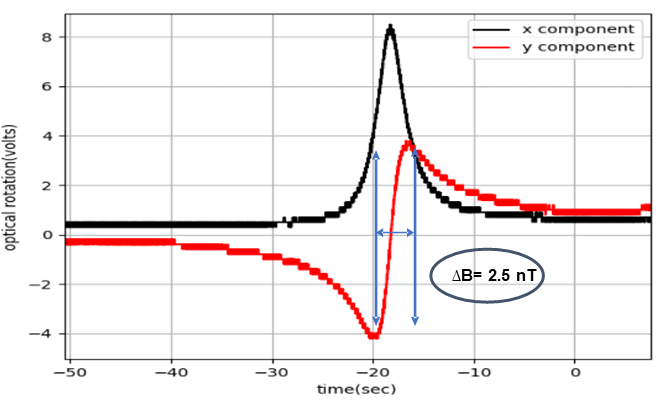
\includegraphics[width=0.5\linewidth]{AM_NMOR}
\caption{AMOR resonance signal with a 5 cm cell containing natural rubidium.Data was acquired by using  a balanced photodiode which demodulated through lock-in amplifier at 9.335 KHz.The observed resonance width is about 2.5 nT}
\end{figure} 
\newpage
\item Force Oscillation Scan\\
Study NMOR signal by sweeping resonance frequency with amplitude modulated light.\\
The magnetometer can be run as a forced oscillator, where a
frequency generator is used to sweep the frequency of the laser amplitude modulator through the NMOR resonance. In this case the applied magnetic field($B_z$) remains fixed during a measurement cycle(pumping and probing).  The experimental setup for this measurement scheme remains almost same as for AM NMOR.The applied magnetic field was about 1  $\mu T $ directed along light propagation direction. 
The measurement was taken by driving an Agilent 33522A function generator to different modulation frequencies in order to find the resonance frequency of the given Rb oscillator. The modulation waveform is a square wave with a duty cycle of 1\%. Since our pump beam is linearly polarized , a modulation at 2 $\Omega_{L}$ is necessary because of the two fold symmetry of alignment state.The typical range of drive frequency is 9.31 KHz to 9.409 kHz for $1\mu T$ field. An unmodulated linearly polarized probe beam is used to analyze the spin response.While the magnetometer response was recorded with a lock-in amplifier, which is connected to balanced photodiode output, demodulating the signal at the drive frequency of the atomic oscillator. 
The center of the resonance is used to determine the Larmor frequency and hence the magnetic field. Figure 5.4 shows the resonance scan where data was taken by setting a function generator to different drive frequencies for the given atomic oscillator.During the scan drive frequencies was working as reference frequencies of the lock-in amplifier. The red and blue data points indicate x and y output respectively. When the modulation frequency is twice the Larmor frequency the x component reaches its maximum and the y component has its zero crossing. In this force oscillation scan the measured resonance width  is 1.67 nT. 
\begin{figure}[h]
\centering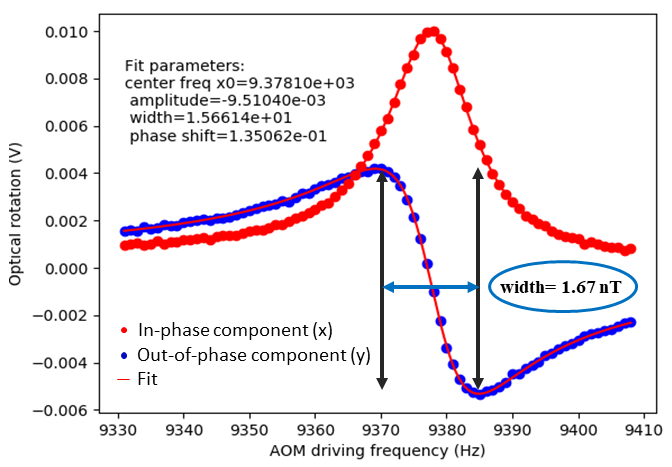
\includegraphics[width=0.5\linewidth]{FM_modulation}
\caption{Optical rotation vs. forced oscillation frequency. NMOR resonance recorded with the 5 cm natural Rubidium cell, square-wave $100\%$ modulation of 1 duty cycle. The x component reaches its maximum and the y component has its zero crossing at $\Omega_m$ = $2\Omega_{L}$.In this case the measured resonance width is 1.67 nT.} 
\end{figure} 
   \end{itemize}
  \newpage
   \section{FID at 0.2 $\mu$T and FID at 
  1 $\mu$T (need to edit) }
  Coherence time indicate the time atoms take to decay spontaneously from excited ground state after removing the pump beam. To measure the coherence time, a pump beam of linearly polarized light is
used to align the atoms along the magnetic field by optical pumping. The pump
beam is then blocked allowing the atoms to relax over time. Optical rotation of the linearly polarized probe beam is used to measure the coherence time. In this measurement optical pumping is done for 0.5 sec. Since at higher field coherence state decays quickly so coherence time get smaller. Figure 5.5 shows the FID signal for  two different field.  At 0.2 $\mu$T field the coherence life time is about 75 ms (Figure 5.5(a)) and when the applied magnetic field is 1 $\mu$T  the coherence lifetime is about 23 ms (Figure 5.5(b)). Since at higher field, FID signal contain less no of oscillation it becomes challenging to extract oscillation frequency precisely and therefore magnetic field. In order to avoid this systematic effect most of the studies reported in this thesis has done at 0.2 $\mu$T.
   \begin{figure}
    \centering
 
    \begin{subfigure}[b]{0.45\textwidth}
        \centering
        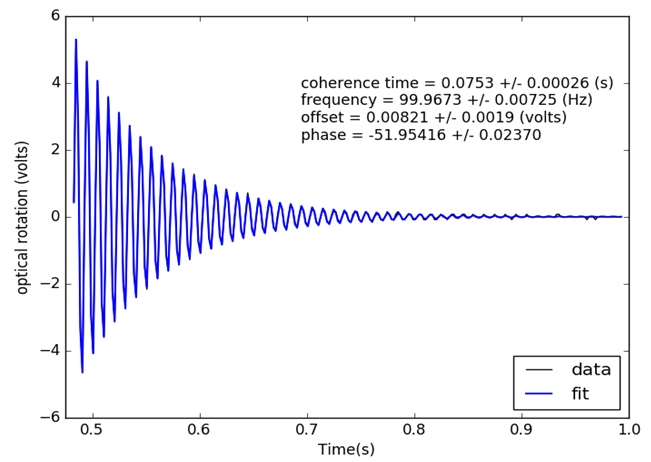
\includegraphics[width=\textwidth]{FID_0_2_micro_tesla}
        \caption{}
        \label{fig:three sin x}
    \end{subfigure}
    \hfill
    \begin{subfigure}[b]{0.45\textwidth}
        \centering
        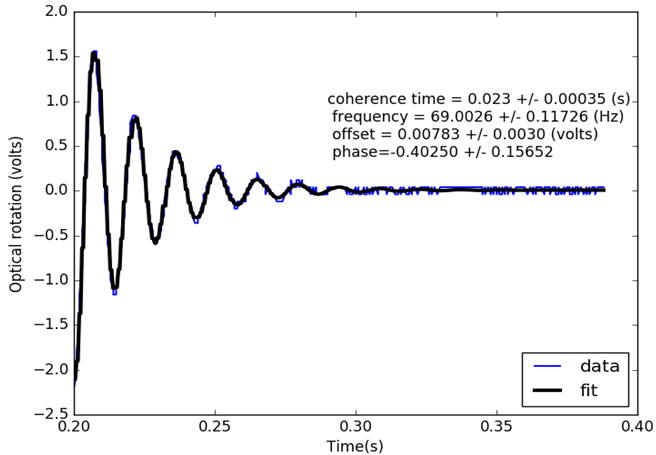
\includegraphics[width=\textwidth]{FID_1_micro_tesla}
        \caption{}
        \label{fig:five over x}
    \end{subfigure}
    \caption{FID NMOR resonances 
obtained with a probe light power of 22 $\mu W$, pump power of 40 $\mu$W. The pump and probe beam both are linearly polarized. FID signal was acquired at 0.2 $\mu$T (a).  FID signal at applied magnetic field 1 $\mu$T (b). The coherence time is larger for smaller field whereas for larger magnetic field the coherence time becomes small. }
    \label{fig:three graphs}
\end{figure}
  \section{long term FID measurement}  
The forced oscillation scans and the single FID shot gives information about the present magnetic field. In order to get information about the change in magnetic field over time, long term data was taken in the FID mode. During this long term process the laser frequency was locked into D1 transition line of Rb-85 using DigiLock 110 laser locking module. A stable power supply was used to run the coil system inside the shield. In order to observe the FID signal, a Tektronix DPO 2014 oscilloscope was connected to X and Y output of output of lock-in amplifier. A python script is used to setup function generator and to trigger DAQ for long term FID measurement. This same python script is also used to grab data continuously from oscilloscope screen to computer. For further data analysis  another python script is used. On the basis of the X
and Y channel recordings, a least-square fit was done for each X and Y pair. The measured oscillation frequency of decaying signal was then convert to magnetic field using equation (4.7). The recorded B-field data vs. time was further used to calculate Allan deviations, getting  information on the deviations from the mean magnetic field vs. integration time (bin size). Measuring magnetic field over long period of time gives us information about the magnetometer performance. Toward this end,we study long term field measurement. Figure 5.6 represents the magnetic field recorder over 4 hours on three different day. Each data points in this graph correspond to single FID scan. The observed field drift is almost same (15 pT) for three days. This measurement was conducted at 0.2 $\mu$T magnetic field.
\begin{figure}[h]
\centering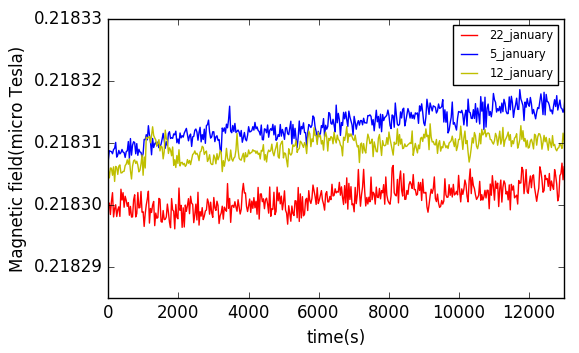
\includegraphics[width=0.85\linewidth]{field_3_day}
\caption{Magnetic field recorded over 4 hours on three different day. The observed field drift is almost same(15 pT) for three days.}
\end{figure}
   \begin{itemize}
   \item summary of statistical error, systematic error, stability via allan deviations.
   \end{itemize}
   \newpage
   \section{Optimization of cycle time} 
   \begin{figure}
    \centering
 
    \begin{subfigure}[b]{0.425\textwidth}
        \centering
        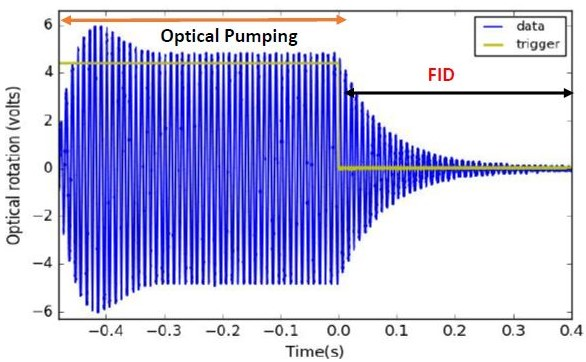
\includegraphics[width=\textwidth]{Capture}
        \caption{}
        \label{fig:three sin x}
    \end{subfigure}
    \hfill
    \begin{subfigure}[b]{0.42\textwidth}
        \centering
        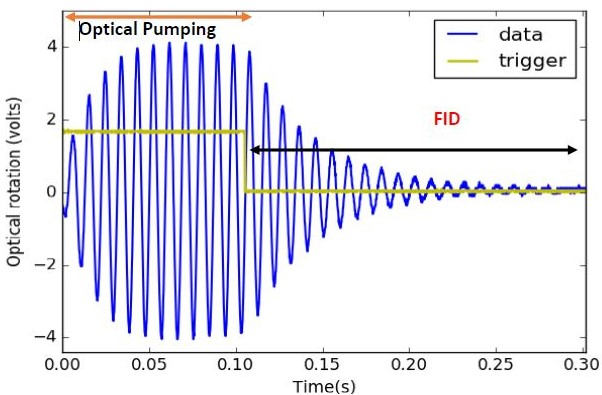
\includegraphics[width=\textwidth]{Capture2}
        \caption{}
        \label{fig:five over x}
    \end{subfigure}
    \caption{(a) FID signal for pump time 0.49 sec and probe time 0.4 sec . (b) FID signal for pump time 0.1 sec and probe time 0.2 sec .Both measurement were conducted at $0.2 \mu$ T magnetic field.}
    \label{fig:three graphs}
\end{figure} 
   \begin{figure}[h]
\centering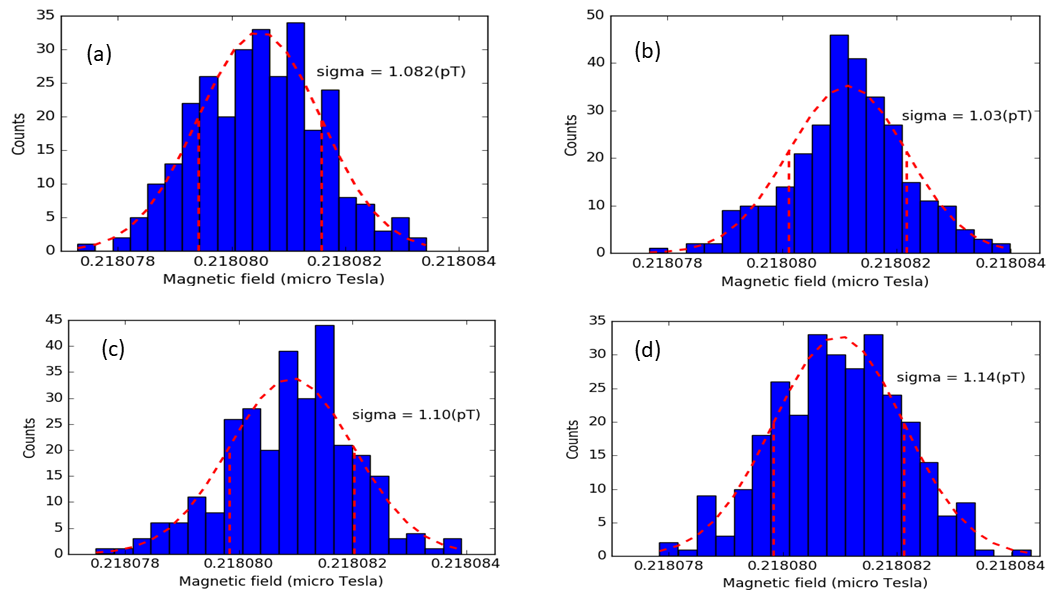
\includegraphics[width=0.75\linewidth]{pump_time}
\caption{Measured B-field vs. time   for different pump time. The longest pump time is 0.49 sec while the shortest pump time is 0.1 sec. No obvious dependency of pump time on  measured magnetic field has been observed during this study}
\end{figure}
In FID NMOR optical pumping is done for polarizing Rb atoms and afterward the spontaneous decay of excited atom is observed. So a complete cycle of FID measurement consist of pump and probe time.Pump time represents the time atoms take to generate a polarized ground state. In this study we were trying to study how long the optical pumping of Rb atom should have continued in order to generate an alignment and optical pumping for long time does make any difference in measuring magnetic field precisely or not.FID signal with 0.49 sec pump time and 0.4 sec probe time has shown in Figure 5.7(a). On the other hand, Figure 5.7(b) shows  the FID signal for 0.1 sec pump time and 0.2 sec probe time. In Figure 5.8 the measured magnetic field in about 300 sec has shown for different pump time. The longer pump time is 0.49 sec and the shorter one is 0.1 sec. It is obvious from the plot that pump time doesn't effect in field precision. However for our Rb magnetometry setup it is not possible to make the pump time shorter than 0.1 sec because this 0.1 sec is the minimum time atoms need to get aligned for making a coherence state after interacting with laser beam. Since the amplitude of FID NMOR signal reach it's maximum while atoms are in coherence state. Thus It is easy to understand coherence state is ready or not by observing the signal amplitude. In Figure 5.7(a) the optical pumping is done for 0.49 sec while signal amplitude reach its maximum over 0.1 sec and after that signal amplitude remains unchanged till 0.49 sec. In this case there is no point to pump more than 0.1 sec.Same situation happens about probe time. If signal amplitude decays so quickly there is no point to set longer probe time.By optimizing pump and probe time we can speed up data acquisition system. After optimization for a single FID scan it only takes 0.35 sec without losing any information. By using this faster data acquisition system it is possible to record multiple FID run with in a short period of time which is helpful to gather more information about magnetic field environment.
\newpage
   \section{current with existing power supply}
   \begin{itemize}
   \item Analysis of current stability.\\
 An Agilent B2962A power supply was used to run the coil system which produce magnetic field inside the shield. In order to develop a highly sensitive magnetometer, it is very important to make use of a highly stable power supply. The idea was to determine the current drifts of the power supplies, mainly based on the fact that the given current supply actually acts as a voltage supply with the output voltage transformed into an output current by a resistor which is sensitive to external influences such as temperature. Figure 5.9 shows the current stability of power supply over 10000 sec. During this time the current only change by 30 nA.  
   \begin{figure}[h]
\centering
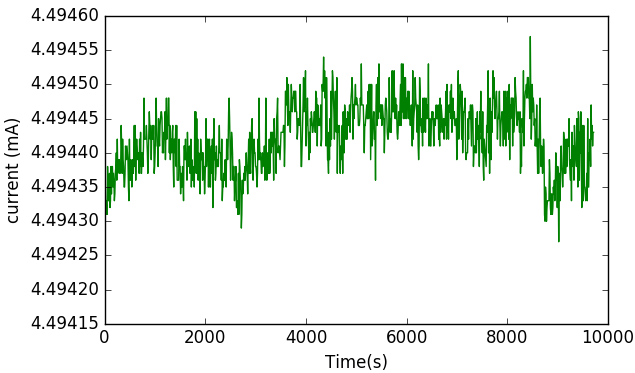
\includegraphics[width=0.8\linewidth]{current}
\caption{Recorded current over 10000 sec using Agilent B2962A power source. During this measurement coil current only changed by 30 nA. }
\end{figure}
   \item Current stability is better than typical measured field changes.
   \item Change in magnetic field due to the change in coil current\\
 A study has been conducted to determine the field change by changing the coil current by a known amount. The main objective of this study is to check the Rb magnetometer performance on magnetic field measurement. During this measurement coil current has been changed by $\pm$ 0.001 mA. As a result a field change of $\pm$ 50  $\mu$T  has been observed. The laser frequency was locked to Rb transition frequency and all other setting kept unchanged. During this study the magnetometer has been operated in FID mode. Figure 5.10 presents the magnetic field change over time for different coil current. For better understanding figure 5.10 has been divide into five different regions. In region-1 magnetic field  has been recorded for 300 sec while the applied current to the Z coil was 4.5 mA. Then in region-2 the applied current to the z coil has been increased by 0.001 mA i.e., total current 4.501 mA and measured the magnetic field for another 300 sec. It is clear from the figure that the field has been changed instantly by $50 \mu$ T due to the changed coil current. Now in region-3, the coil current has been reduced to 4.5 mA and measured field for 300 sec. After that the coil current has been decreased by 0.001 mA. As a result the field also decreased by $50 \mu$T in this region.Finally in region-5 the coil current has been set to 4.5 mA again and observed the corresponing quick change in field.

   \begin{figure}[h]
\centering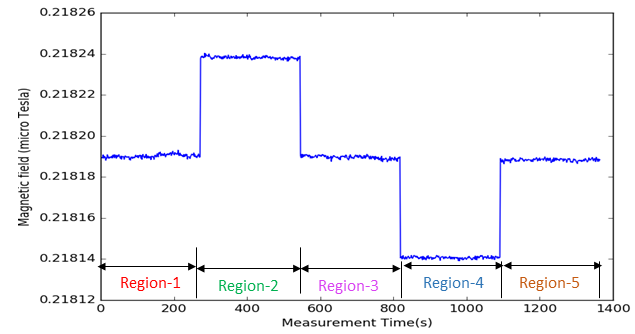
\includegraphics[width=0.7\linewidth]{field_change_with_current}
\caption{The change in magnetic field  by changing coil current has been studied over 1400 sec. The blue line on different regions of the graph displays the measured magnetic field corresponding to the change in coil current. }
\end{figure}
   \end{itemize}
   \section{degaussing studies}  
   \begin{itemize}
   \item different degaussing schemes(changing sample rate)\\
Degaussing process is done in order to avoid the environmental perturbation and reduce any remnant field inside the four layer $\mu$ metal magnetic shield \cite{doi:10.1063/1.2713433}. For our degaussing system we are using an envelope function which has $1*10^6$ points.Degaussing is complete after $5*10^6$ points.Sample rate affects how quickly we move through this waveform. A detailed analysis of NMOR signal by changing the degaussing parameter could give us some information about the goodness of degaussing procedure. Toward this end, a study has been carried out to determine  the dependency of the resonance width on the sample rate. In this case, data was acquired by sweeping the magnetic field near zero field. Before each measurement degaussing the innermost layer of shield has done. During this measurement only one degaussing parameter,sample rate, was varied in order to study the effect of degaussing parameter on magnetic field measurement.  Optical rotation as a function of magnetic field for different sample rate has shown in Figure 5.10. The resonance width $\Delta B$, the difference between two peak of the dispersive curve, changed for different sampling rate. It can be seen from figure 5.10 that, the resonance width is about 0.49 nT for sample rate 10000 sample/sec and the resonance width is 0.38 nT for sample rate 80000 sample/sec. Figure 5.11 shows the resonance width as a function of sample rate. It is obvious from the graph that the resonance width becomes narrower for larger sample rate.    
   
   \begin{figure}[h]
\centering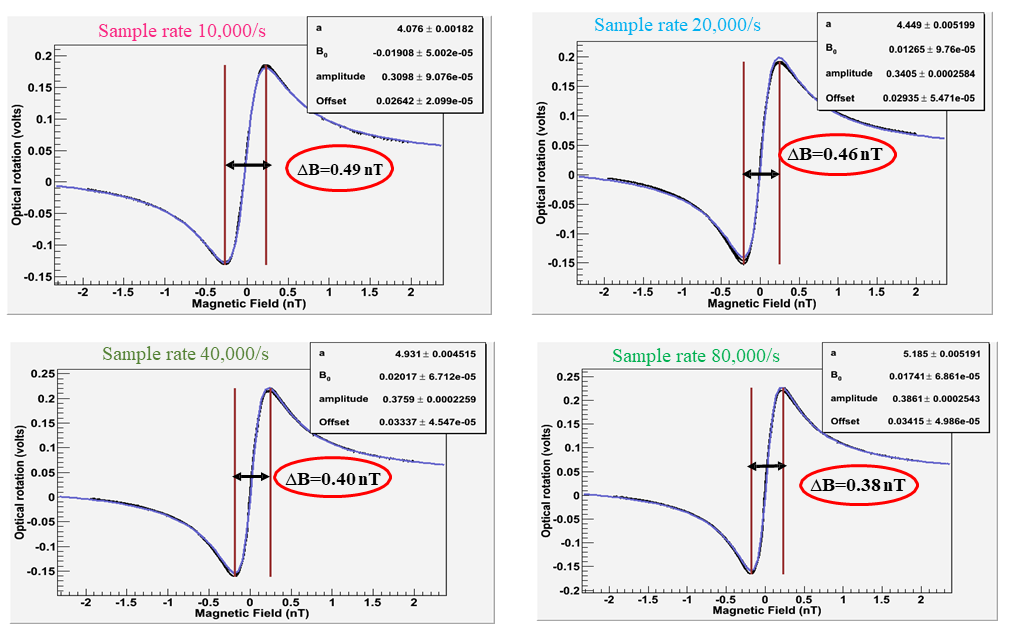
\includegraphics[width=0.65\linewidth]{sample_rate}
\caption{ Optical rotation vs. measured B-field   for different sample rate.The resonance width is narrower(0.38 nT) for higher sample rate(80000 sample/sec) whereas the resonance width becomes broaden (0.49 nT) for lower sample rate. }
\end{figure}
\begin{figure}[h]
\centering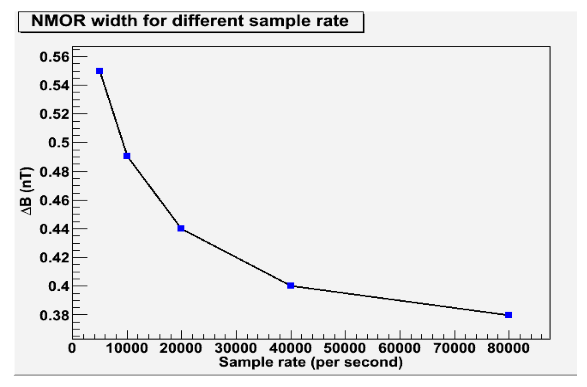
\includegraphics[width=0.6\linewidth]{field_vs_sample_rate}
\caption{Resonance width vs. sample rate. Resonance width decreases with increasing sample rate.When sample rate is 5000 sample/sec the observed resonance width is 0.55 nT. On the other hand the resonance width is 0.38 for sample rate 80000 sample/sec.  }
\end{figure}
\newpage
   \item Ramp field up/down \\
  During this study the magnetometer has been operated in FID mode at 0.2 $\mu$T field. The recorded magnetic field over 2200 sec has been showed in Figure 5.13(a). No degaussing has been done during this measurement. It can be seen from the figure the magnetic field increase linearly for first 300 sec then showed a decrease in field. The field was pretty stable between 600 sec and 1800 sec and after that the field showed a rapid increase.The overall field change is about 15 pT during the measurement.Data was acquired by ramping $B_z$  from  0.2 $\mu$T to 10 $\mu$T then again set it to 0.2 $\mu$T and collect FID signal. By doing this field ramping we intentionally perturb the magnetic field environment inside the shield. After this field ramping the long term field measurement has been conducted for another 2200 sec. In this case, the field showed a downward drift of about 35 pT. Thus field ramping has been changed the magnetic field environment inside the magnetic shielding.
   \begin{figure}
    \centering
 
    \begin{subfigure}[b]{0.425\textwidth}
        \centering
        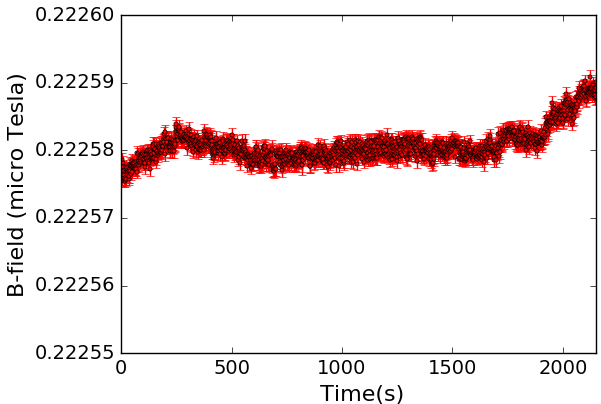
\includegraphics[width=\textwidth]{ramp_1}
        \caption{}
        \label{fig:three sin x}
    \end{subfigure}
    \hfill
    \begin{subfigure}[b]{0.42\textwidth}
        \centering
        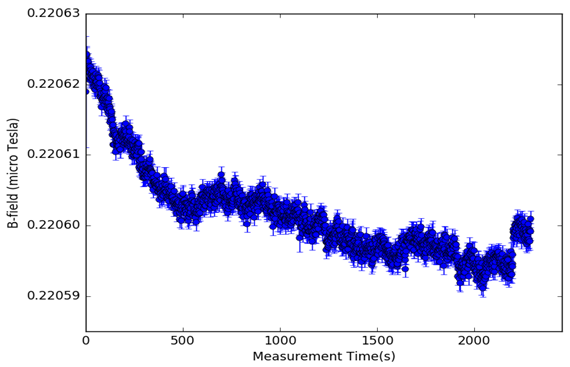
\includegraphics[width=\textwidth]{ramp_2}
        \caption{}
        \label{fig:five over x}
    \end{subfigure}
    \caption{ FID signal at $B_z=0.2 \mu$T magnetic field.(a) no degaussing (b) ) Ramp $B_z$  from  0.2 $\mu$T to 10 $\mu$T then again set it to 0.2 $\mu$T and collect FID signal.}
    \label{fig:three graphs}
\end{figure}
   
   \item degaussing second innermost shield effect in field drift.\\
   After doing transverse field study (applying current to X and Y coil along with Bz coil) magnetic field environment was pretty unstable. Figure 5.14(a) shows about 50 pT drift in magnetic field in 4000 sec. In order to cancel background field inside shield degaussing innermost layer of $\mu$ metal is done but it doesn't help to solve field drift problem. Then degaussing the 2nd innermost layer of shield is done which solve the field drift problem. Since the end cap of the innermost shield layer is not in use some background field leaked into 2nd layer which was causing the drift in field. So by degaussing the 2nd layer of shield canceled background field and field becomes so stable (Figure 5.14 (b)).
   
  \begin{figure}
    \centering
 
    \begin{subfigure}[b]{0.45\textwidth}
        \centering
        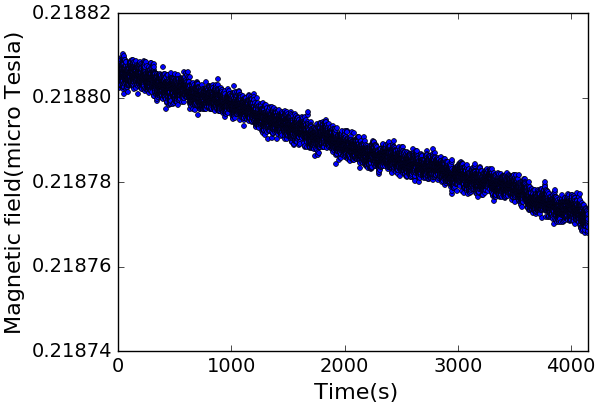
\includegraphics[width=\textwidth]{before_degaussing}
        \caption{}
        \label{fig:three sin x}
    \end{subfigure}
    \hfill
    \begin{subfigure}[b]{0.45\textwidth}
        \centering
        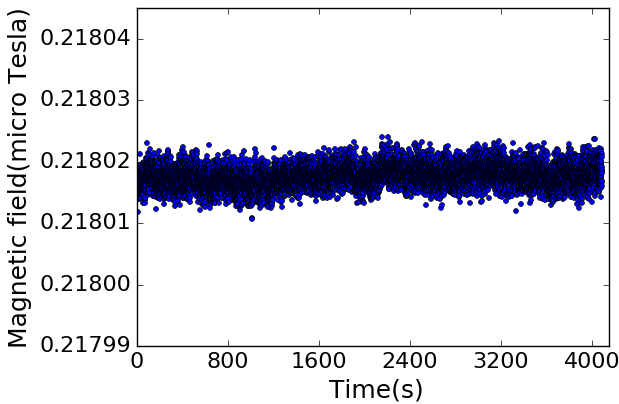
\includegraphics[width=\textwidth]{after_degaussing}
        \caption{}
        \label{fig:five over x}
    \end{subfigure}
    \caption{ Magnetic field recorded over 3 hours. (a) The stability of magnetic field without performing any degaussing. A downward field drift of about 45 pT  has observed in this case (b) magnetic field stability after degaussing the 2nd innermost layer of magnetic shielding. Only a couple pT field drift has observed in this case.}
    \label{fig:three graphs}
\end{figure}
   \end{itemize}
   \newpage
   \section{Laser tuning} 
   \begin{itemize}
   \item effect of careful tuning\\
	The main purpose of this study is to understand the importance of laser tuning on coherence life time of excited atoms. During the study optical pumping is done to polarize the rubidium atom and hence produce coherence state. When the laser light  is  exactly tuned to resonance with the atomic transition, the lifetime of coherence state becomes longer and the amplitude of resonance signal reaches its maximum. On the other hand coherence state decay  quickly when laser frequency detunes from atomic transition. In this case, the signal amplitude reduces due to frequency detuning. Figure 5.15 shows the effect of laser tuning on coherence lifetime. For proper laser tuning the observed coherence time is 68 ms (a) whereas for bad tuning coherence time reduces to 59 ms (b). Since  longer coherence time and larger signal amplitude indicate better frequency precession and therefore precise field measurement it is very important to make sure the laser tuning has done carefully.
   \begin{figure}
    \centering
 
    \begin{subfigure}[b]{0.45\textwidth}
        \centering
        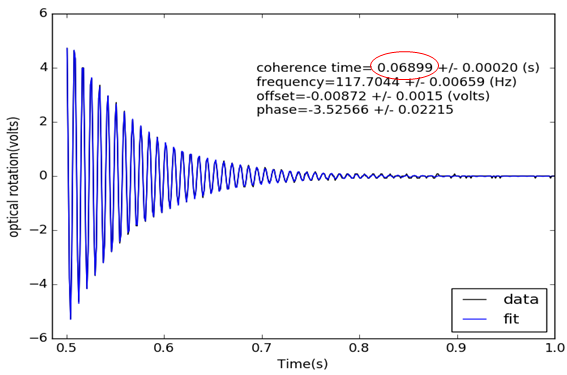
\includegraphics[width=\textwidth]{perfect_tuning}
        \caption{}
        \label{fig:three sin x}
    \end{subfigure}
    \hfill
    \begin{subfigure}[b]{0.45\textwidth}
        \centering
        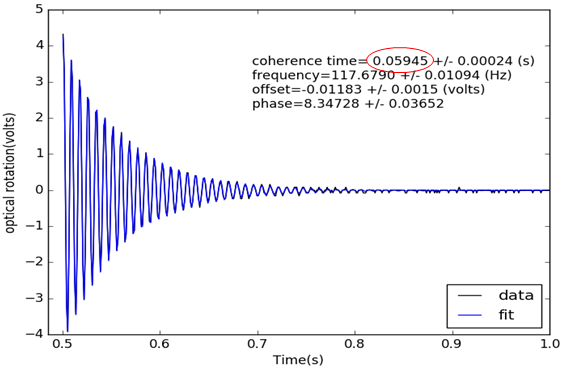
\includegraphics[width=\textwidth]{bad_tuning}
        \caption{}
        \label{fig:five over x}
    \end{subfigure}
    \caption{(a) Recorded FID signal while laser is perfectly tuned to atomic transition frequency. (b) FID resonance signal when laser is slightly detuned from transition frequency.}
    \label{fig:three graphs}
\end{figure}
   \item problem with drift of tune\\
   For studying long term stability data was taken for about 12 hours.Laser was locked to D1 transition line of Rb using Digilock laser locking software. Figure 5.15 shows 120 pT observed drift in magnetic field over 12 hours. Although DAVLL was in use laser frequency was not locked for 12 hours. As a result laser tuning moved due to mode hoping which causes the drift. The current laser locking system only works perfectly for maximum 4 hours. The possible reason for this mode hoping is the Polarizing beam splitting cube of our DAVLL system \cite{principles}. The disadvantage of using this type of PBS is that they show flaky optical behavior over longer times.
   \begin{figure}[h]
\centering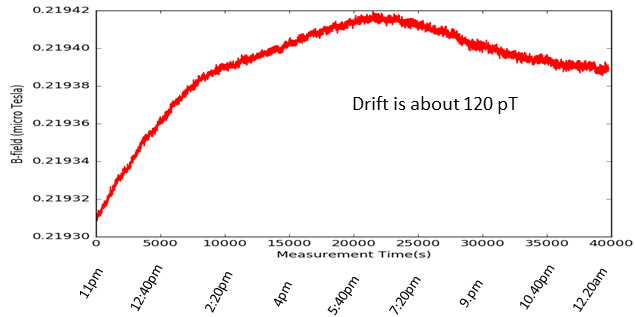
\includegraphics[width=0.5\linewidth]{field_drift}
\caption{Magnetic field recorded over 12 hours.In this measurement the observed field drift is about 120 pT.}
\end{figure}
\item manual tuning\\
   During this study frequency of laser light is tuned to atomic transition maximize optical rotation.The laser tuning was adjusted manually time to time for maintaining same signal amplitude during measurement .The main objective of this study is to check the observed drift in field measurement is the real field drift or the magnetometer drift due to the mode hoping. Instability of laser locking system due to the poor performance of PBS which is used in DAVLL system is the probable reason behind this mode-hoping. According to figure 5.17~ (b) we can say that during this measurement the amplitude of FID NMOR was pretty stable except small fluctuations over 20000 sec . The observed small fluctuation is due to the manual adjustment while keeping the laser frequency tuned to atomic transition over long period of time. Obtaining stable signal amplitude is a indication that laser is not drifting to much. Although laser frequency was not drifting a lot during  the measurement, still there is a  drift in magnetic field (Figure 5.17 (a)). The overall drift is about 20 pT over 20000 sec. So it can be conclude that the drift in laser frequency is not the main reason behind this induced field drift. 
   
    
   \end{itemize}
   \begin{figure}
    \centering
 
    \begin{subfigure}[b]{0.45\textwidth}
        \centering
        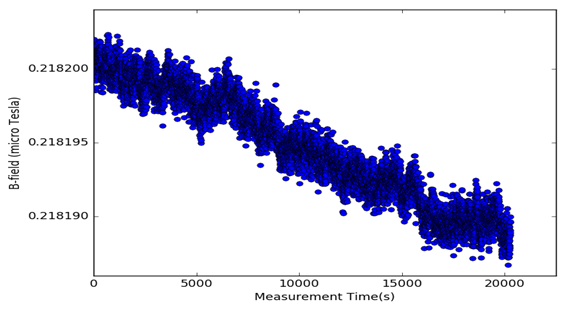
\includegraphics[width=\textwidth]{manual_tuning}
        \caption{}
        \label{fig:three sin x}
    \end{subfigure}
    \hfill
    \begin{subfigure}[b]{0.45\textwidth}
        \centering
        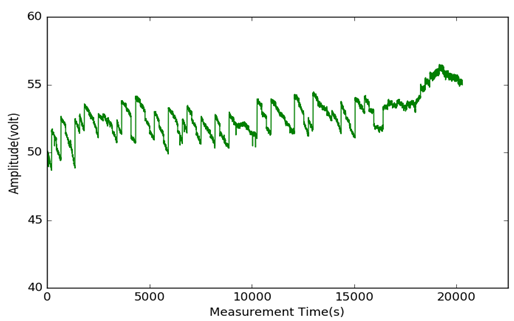
\includegraphics[width=\textwidth]{amplitude_manual_tuning}
        \caption{}
        \label{fig:five over x}
    \end{subfigure}
    \caption{(a) magnetic field vs. time. (b) amplitude of recorded FID NMOR signal over 20000 sec. During this study laser tuning is maintained manually}
    \label{fig:three graphs}
\end{figure}
   \section{Optimization of pump and probe beam power} 
 A study has been performed to determine how optimization of the pump and probe beam power effect on precise field measurement.  During this study, the magnetometer has operated in FID mode.  A  linearly polarized probe beam has been used to analyze the spin response. In figure 5.18 the measured magnetic field has been displayed for two different  Probe beam power. Figure 5.18 (a) present the measured field over 100 sec with 15 $\mu$ W probe power while figure 5.18(b) display the measured field over 100 sec for probe power 30 $\mu$W. In both cases, the pump beam power has been kept unchanged ($5\%$ duty cycle). Each blue points in this graph represent a single FID scan. As can be seen from figure 5.18 the magnetic field is more scattered for high beam power. Precession width is about $15$ pT for probe beam power 30 $\mu$W while for low beam power(15 $\mu$W) the precession width is about $7$ pT. It can be concluded lower probe beam power is better for precession  magnetometry because the narrower the precession width more sensitive the magnetometer is . Although low probe beam power is better for precise field measurement, it's hard to work with because of the dimness of light.\\
  \begin{figure}
    \centering
 
    \begin{subfigure}[b]{0.45\textwidth}
        \centering
        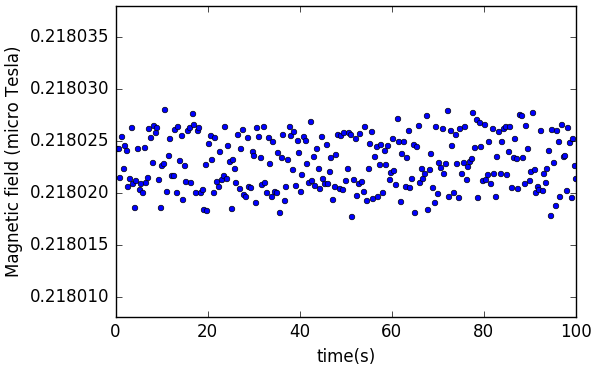
\includegraphics[width=\textwidth]{beam_power_less}
        \caption{}
        \label{fig:three sin x}
    \end{subfigure}
    \hfill
    \begin{subfigure}[b]{0.45\textwidth}
        \centering
        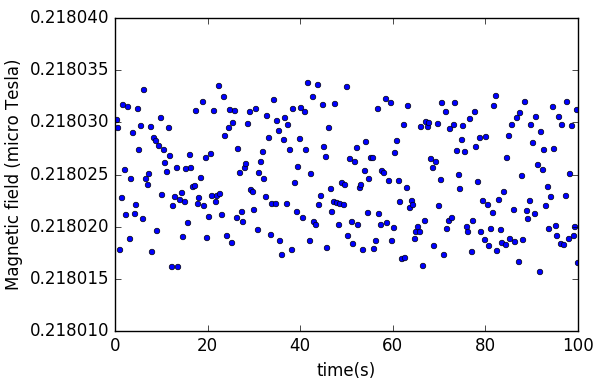
\includegraphics[width=\textwidth]{beam_power_double}
        \caption{}
        \label{fig:five over x}
    \end{subfigure}
    \caption{ Magnetic field as a function of time for different power of probe beam.(a) measured magnetic field with probe beam power 15 $\mu$w. Precession width is about $7$ pT (b) measured magnetic field with precession width $15$ pT for probe beam power 30 $\mu$w.}
    \label{fig:three graphs}
\end{figure}
Another study has been conducted to understand the influence of pump beam power on precession magnetometry. During this study, the probe beam power has kept unchanged while pump power has changed. In this measurement data has been acquired by running the magnetometer in FID mode. In FID mode amplitude modulation of pump beam has been done by using a AOM.  So the pump beam power can be change by changing the duty cycle of square wave modulation. When duty cycle is set to $5\%$ the pump beam power is 40 $\mu$W and for $16 \%$ duty cycle power is 128 $\mu$W. The histogram of measured magnetic field for different pump beam power has been showed in figure 5.19. The precession width (sigma) become larger for higher duty cycle while it becomes narrower for small duty cycle. In the case of 5$\%$  duty cycle precession width is about 2.3 pT  5.19 (a) and for 16 $\%$ duty cycle the spread is about 4.6 pT. It is clear from the plot that, at higher duty cycle data points are not statistically distributed.  When a pump beam with a higher duty cycle is used  in precession magnetometry, the NMOR  signal amplitude increase accordingly. But it has been observed that error in frequency measurement also increases with higher signal amplitude which was not expected. A strong correlation between magnetic field and phase of the NMOR signal also has been observed for higher pump power. So it can be concluded that using higher duty cycle could induce more systematic errors in field measurement which led to the next study.
 \begin{figure}
    \centering  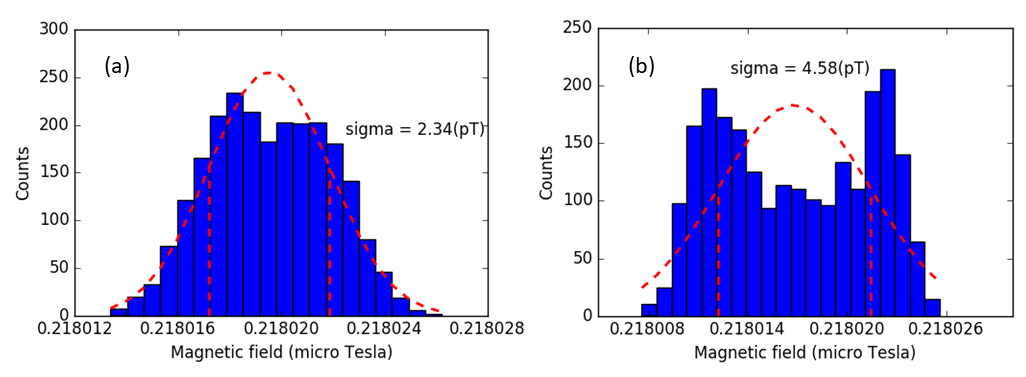
\includegraphics[width=\textwidth]{pump_beam}
    \caption{ Magnetic field vs. time for different pump beam power.(a) measured magnetic field with duty cycle $5 \%$. Precession width is about $2.3$ pT (b) measured magnetic field with Precession width $4.6$ pT for  16 $\%$ duty cycle.}
    \label{fig:three graphs}
\end{figure}
   \section{Systematic error check in frequency measurement in FID mode} 
   \subsection{How far the reference frequency of lock-in amplifier should set to measure field correctly}
  
  In FID NMOR the atomic sample is polarized once by optical pumping and then observed the spontaneous decay of excited atom while the pump beam is off.In order to capture the FID signal correctly, the reference frequency of lock-in amplifier is normally set to about 100 Hz apart from the resonance frequency. In this study we kept all other setting fixed only changed the Lock-in reference frequency and observed the effect of that on field measurement study. The measurement was conducted at $0.2\mu$ T field. The FID signal for different reference frequency of Lock-in amplifier has shown in Figure 5.20. In the case of Figure 5.20 (a) the reference frequency of Lock-in was set to 1943.9 Hz(90 Hz far from resonance frequency). On the other hand for Figure 5.20 (c) the reference frequency of Lock-in was set to 2015 Hz(20 Hz far from resonance frequency). In this study the resonance frequency is 2035 Hz. In Figure 5.21 the measured magnetic field over 35 sec for different lock-in reference frequency has shown. It is obvious from the plot that if we set reference frequency very close to resonance frequency magnetic field start to oscillate. The exact reason behind this observed field oscillation remains unknown. We are thinking that when lock-in reference frequency is set very close to resonance frequency the fit function might fail to fit data properly due to the less zero crossings. So it seems like a systematic effect on field measurement rather than a real fact.
 \begin{figure}
    \centering
    \begin{subfigure}[b]{0.4\textwidth}
        \centering
        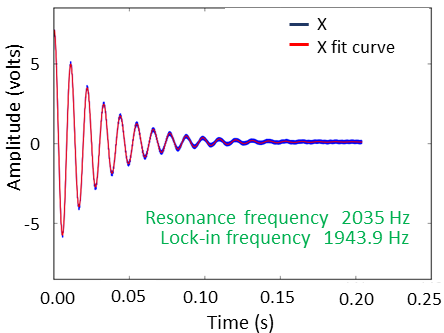
\includegraphics[width=\textwidth]{reference_frequency1}
        \caption{}
        \label{fig:three sin x}
    \end{subfigure}
    \hfill
    \begin{subfigure}[b]{0.4\textwidth}
        \centering
        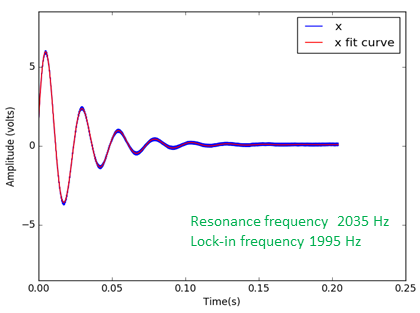
\includegraphics[width=\textwidth]{reference_frequency3}
        \caption{}
        \label{fig:five over x}
    \end{subfigure}
    \begin{subfigure}[b]{0.4\textwidth}
        \centering
        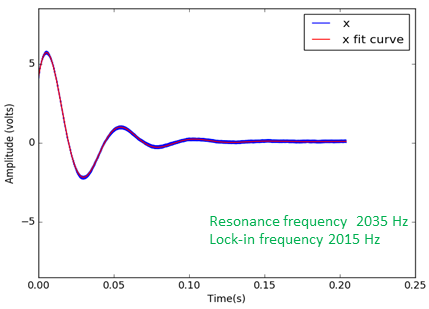
\includegraphics[width=\textwidth]{reference_frequency2}
        \caption{}
        \label{fig:five over x}
    \end{subfigure}
    \caption{FID signal for different reference frequency of Lock-in amplifier while the resonance frequency was 2035 kHz.(a) reference frequency was set to 100 Hz far from resonance (b) difference between resonance and reference frequency is 40 Hz,(c) reference frequency was set to 2015 Hz while resonance frequency 2035 Hz. }
\end{figure}
\begin{figure}[h]
\centering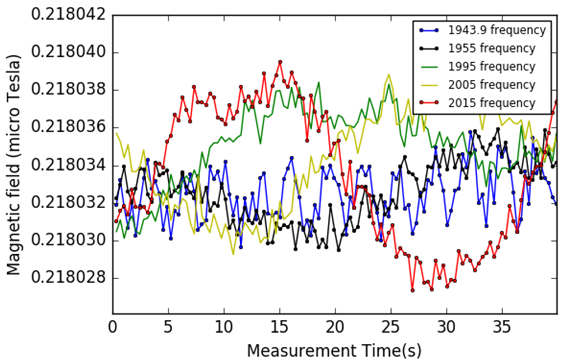
\includegraphics[width=0.8\linewidth]{reference_frequency}
\caption{Measured magnetic field for different lock-in reference frequency.The red curve represents measured magnetic field when reference frequency was set to 2015 Hz which is 20 Hz far from resonance frequency. The blue curve shows magnetic field for lock-in reference frequency 1943.9 Hz.}
\end{figure}
\begin{figure}[h]
\centering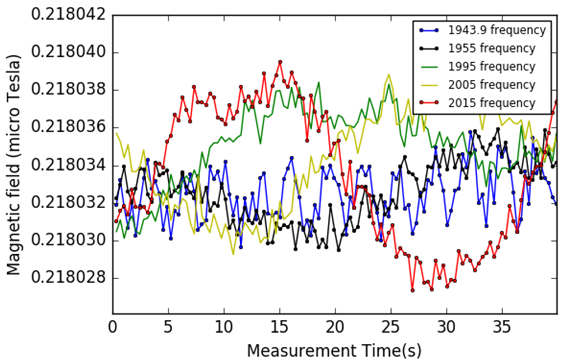
\includegraphics[width=0.8\linewidth]{reference_frequency}
\caption{Measured magnetic field for different lock-in reference frequency. The red curve represents measured magnetic field when reference frequency was set to 2015 Hz which is 20 Hz far from resonance frequency. The blue curve shows magnetic field for lock-in reference frequency 1943.9 Hz.}
\end{figure}
\begin{figure}[h]
\centering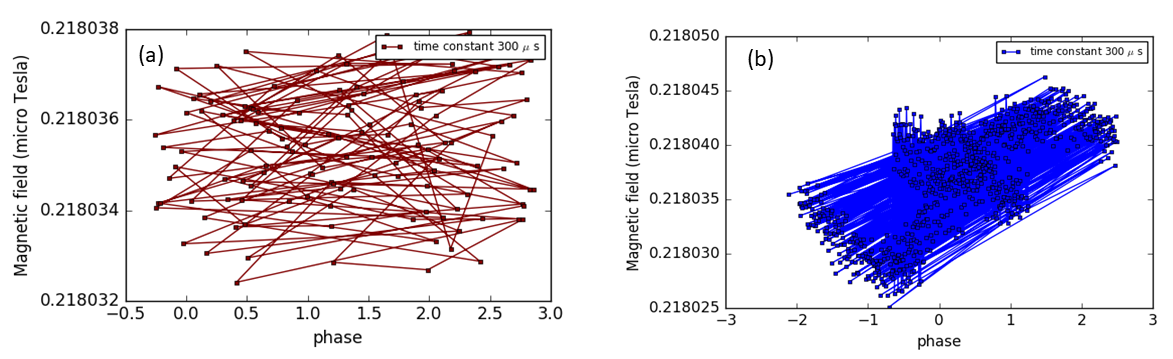
\includegraphics[width=0.8\linewidth]{phase}
\caption{Measured magnetic field for different lock-in reference frequency.The red curve represents measured magnetic field when reference frequency was set to 2015 Hz and field for lock-in reference frequency 1943.9 Hz.}
\end{figure}
\newpage
   \begin{itemize}
   \item effect of lock-in time constant\\
  A SRS-830 lock-in amplifier is used to grab FID NMOR signal which was connected to the output of balanced photodiode. Table 4.1 represents all settings for FID NMOR. In this study the systematic effect of changing locking amplifier time constant on magnetic field measurement has been discussed. Figure 5.22  shows the histogram of measured magnetic field for two different time constant of lock-in amplifier while all other settings is same. In the case of Figure 5.22 (a) the lock-in time constant is 1 ms and figure 5.22 (b) shows the histogram of magnetic field for time constant 300 $\mu$s. Here sigma is representing the precession width of field. It can be seen from the figure that the calculated sigma is larger for time constant 1 ms compared to 300 $\mu$s. This measurements was conducted at 0.2 $\mu$T field. The resonance frequency and lock-in reference frequency are 2035 Hz and 1943 Hz respectively.
   \begin{figure}
    \centering
    \begin{subfigure}[b]{0.4\textwidth}
        \centering
        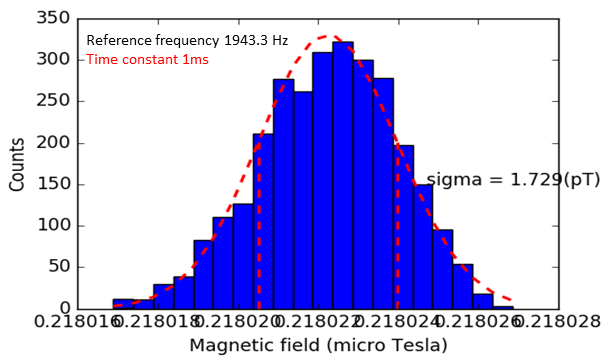
\includegraphics[width=\textwidth]{time_constant}
        \caption{}
        \label{fig:three sin x}
    \end{subfigure}
    \hfill
    \begin{subfigure}[b]{0.4\textwidth}
        \centering
        \includegraphics[width=\textwidth]{time_constant_300micro_sec}
        \caption{}
        \label{fig:five over x}
    \end{subfigure}
    \caption{Histogram of measured magnetic field for different time constant of lock-in amplifier. (a) lock-in time constant was set to 1 ms (b) for lock-in time constant 300 $\mu$s. }
\end{figure}
    \item timing drift in Tektronix oscilloscope clock
   \end{itemize}
   \newpage
   \section{Calculation of Allan deviation} 
   Allan variance is used to investigate long term stability.In this case, the Allan deviation was calculated in order to determine the deviation of the average field value for a given integration time as a function of the integration time\cite{doe:website2}. Consider a time series of measurements $y_i$ is acquired at times $t_i$ and  a subset of N data points are present.
 \begin{equation}
 \bar{y}_{n}= \sum_{i=(n-1)N+1}^{nN} \frac{y_i}{N} 
 \end{equation}

The Allan deviation can be express as
\begin{equation}
\sigma_y(\tau)=\sqrt{\sigma_y^2(\tau)}=Var_y(\tau)
\end{equation}
Where $\sigma_y$ is the Allan deviation, $\tau$ the time of each frequency estimate and $Var_y$ is the variance of the observed data points.
\begin{equation}
{\sigma_y^2(\tau)}=\frac{1}{2}(\bar{y}_{n+1}-\bar{y}_{n})
\end{equation}
where $\bar{y}_{n}$ is the fractional frequency average over the observation time $\tau$.
Allan deviation formula for sinusoidal waveform:
Suppose
\begin{equation}
y(t) = A\cos (\omega t + \phi)
\end{equation}
The average of this function over a time-interval  is
\begin{equation}
\bar{y}_{n}=\frac{2A}
{\tau \omega}
cos(\omega(t_n +\frac{\tau}{2})+\phi)sin(\frac{\omega \tau}{2})
\end{equation}
and
\begin{equation}
\bar{y}_{n+1}=\frac{2A}
{\tau \omega}
cos(\omega(t_{n+1} +\frac{\tau}{2})+\phi)sin(\frac{\omega \tau}{2})
\end{equation}
Now from equation(5.5) and (5.6) we can write
\begin{equation}
\bar{y}_{n+1}-\bar{y}_{n}=\frac{2A}
{\tau \omega}sin(\frac{\omega \tau}{2})[cos( \omega(t_{n+1} +\frac{\tau}{2})+\phi)-cos(\omega(t_n +\frac{\tau}{2})+\phi)]
\end{equation}
Thus Allan deviation can be written as

\begin{equation}
{\sigma_y^2(\tau)}=\frac{1}{2}(\bar{y}_{n+1}-\bar{y}_{n})=(\frac{4A}
{\tau \omega}sin^2(\frac{\omega \tau}{2}))^2 \sin^2     (\frac{\omega(t_{n+1} +t_{n}+\tau)}{2})+\phi)
\end{equation}
For a large number of randomly
distributed tk the average of the sine-squared function is
\begin{equation}
\sin^2    (\frac{\omega(t_{n+1} +t_{n}+\tau)}{2})+\phi)=\frac{1}{2}
\end{equation}
We therefore find that
\begin{equation}
{\sigma_y^2(\tau)}=(\frac{2A}
{\tau \omega}sin^2(\frac{\omega \tau}{2}))^2
\end{equation}
\begin{figure}[h]
\centering\includegraphics[width=0.6\linewidth]{allan_plot}
\caption{Allan deviation vs. averaging time(s)}
\end{figure}
In FID mode, the resonance signal looks like a decaying sine wave. By fitting the NMOR signal with a damped sine wave the oscillation frequency has been extracted and finally this oscillation frequency has been translated to field.The Allan deviation of the measure field has been plotted in Figure 5.23.
\newpage
  \section{study the effect of room temperature in magnetic field} 
  \begin{figure}[h]
\centering\includegraphics[width=0.6\linewidth]{temp}
\caption{Allan deviation vs. averaging time(s)}
\end{figure}
\newpage
   \section{Study magnetometer performance with transverse field}  
   
\begin{figure}[h]
\centering\includegraphics[width=0.5\linewidth]{tilted_field_amp_vs_angle}
\caption{The amplitude of the FID NMOR signals recorded at $2\Omega_L$ vs. the tilt angle of the magnetic field in xz-plane}
\end{figure}
 The magnetometric method based on FID NMOR is a very sensitive technique of magnetic field measurements. Those measurements are scalar, i.e., the position of a given resonance depends only on the magnitude not the direction of the magnetic field. However, the relative magnitudes of the FID NMOR resonances could have some dependency on the magnetic field direction. Thus there is a possibility to get some information about the direction of the magnetic field by doing a detailed analysis of the FID NMOR signal.  For this reason, the dependency of the FID NMOR signal on the magnetic field direction has studied here.  In this Rb NMOR magnetometry setup the rubidium atoms interacted with a z-directed laser light beam which is linearly polarized
along the y axis. In the FID NMOR technique, the magnetic field is generally directed along the light propagation direction and the resonance occurs at $2\Omega_L$.  This effect can be explained by considering that the polarization returns to its original state after a 180° rotation because of the two-fold symmetry of the optically pumped state. As a result, the optical rotation induced by the rotating linear dichroism is periodic at twice the Larmor frequency.
We have observed that Resonances in nonlinear magneto-optical rotation with amplitude modulated light by tilting the magnetic field at angles away from the direction of light propagation while operating the Rb magnetometer in FID mode. When the field is tilted in the plane perpendicular to the light polarization direction an resonance appears at $2\Omega_L$. In this case no additional resonance appears for modulation frequency $\omega_L$. The amplitude of the resonance signal decreases with increasing tilt angle. Figure 5.24 shows the amplitude of the FID signal for the magnetic field tilted in the xz plane at various angles to the light propagation direction at modulation frequency $2\Omega_L$.
However, We also observed that by tilting the field direction toward the light polarization direction a new resonance occurs at $\Omega_L$ along with the main resonance at $2\Omega_L$. The resonance signal recorded at $\Omega_L$ contains two frequency components. Figure 5.25 (b) display the FFT of resonance signal for tilt angle $15\degree$ where two peak corresponds to two frequency components . The amplitude of  resonance signal at $2\Omega_L$  decreases as the angle between magnetic field (B) and the light propagation direction increases while the amplitude of new resonance  increases with increasing tilt angle at $\Omega_L$. Figure 5.25(a) shows the resonance amplitude at $\Omega_m=2\Omega_L$ keep decreases with increasing tilt angle in yz plane while  the resonance amplitude measured at $\Omega_m=\Omega_L$ keep increase till $30\degree$ and after that amplitude start to decrease and reaches zero when the magnetic field is directed along the y axis.Consider a two-level system F=1→F=0 and the quantization vector is directed along the magnetic field. When the magnetic field is tilted in the yz plane, the light-polarization axis is perpendicular to the magnetic field. In this case the linearly polarized light containing two circularly polarized components can only create the coherence state between magnetic sublevels $m = ±1$ . Since the transition frequency between these two consecutive Zeeman energy sublevels is $2\Omega_L$  the resonance appears only at this frequency. However, when the magnetic field is tilted  in the xy plane, the light is a linear superposition of polarizations parallel and perpendicular to the magnetic field. In this case, the light can create coherences between sublevels with $m=1$ and $m=2$, so resonances are observed at both $\Omega_L $ and $2\Omega_L$.

\begin{figure}
    \centering
   \begin{subfigure}[b]{0.45\textwidth}
        \centering
        \includegraphics[width=\textwidth]{amp_tiltangle}
        \caption{}
        \label{fig:y equals x}
    \end{subfigure}
    \hfill
     \begin{subfigure}[b]{0.45\textwidth}
        \centering
        \includegraphics[width=\textwidth]{tansverse_field_fft}
        \caption{}
        \label{fig:three sin x}
    \end{subfigure}
    \caption{(a) The amplitude of the FID NMOR signals as a function of tilt angle recorded at $\Omega_L$ and $2\Omega_L$ vs. the tilt angle of the magnetic field in the plane defined by the light-polarization and light propagation vectors(yz-plane). (b) FFT of FID NMOR signal in the presence of trensverse field.}
\end{figure}


\chapter{}
\section{Conclusion}
\section{Future work}
\begin{itemize}
\item	FEMM simulation of z-coil 	Homogeneity of z-coil in this shielding configuration is not known or measured.  (Never measured with endcaps of innermost shield removed.)
\begin{itemize}
\item Probably this is to compare with Junyao’s coil and its homogeneity

\item
Can also measure homogeneity of z-coil in shield – it has been done before and I recall that it is homogeneous at $\% $level when in shield with basic degaussing (not our present degaussing system).
\end{itemize}
\item
Study magnetometer performance with Junyao's coil inside shield. 
\begin{itemize}
\item	The idea here is to show whether decoupling the coil from the shield has any impact on long-term stability.
 \item removing the lock-in amplifier
\end{itemize}
\end{itemize}
\newpage
\printbibliography
\end{document}


